\documentclass[dvipsnames,aspectratio=169]{beamer}
%\usepackage{fontspec}
%\setmainfont{Ubuntu}
\usepackage[medium]{ubuntu}  
\usepackage{beamerthemeinsight/insight}
\usepackage{tabularx}
\usepackage{ragged2e}
\usepackage{stackengine}


\usepackage{url}
\usepackage{xcolor}
\usepackage{colortbl}
\usepackage{graphicx}
\usepackage{listings}
%\input{mznlisting}
%\lstset{language=Mzn}

\usepackage{tikz}
\usetikzlibrary{calc}
\usetikzlibrary{positioning}
\usetikzlibrary{shapes}
%\usetikzlibrary{graphs,graphdrawing,quotes}
%\usegdlibrary{trees}
%\usegdlibrary{layered}

\tikzset{activity/.style={fill=insight-royalblue!20,draw=black!40}}
\tikzset{operator/.style={fill=insight-lime!20,draw=black!40}}
\tikzset{moreactivity/.style={fill=insight-royalblue!10,draw=black!40}}
\tikzset{moreoperator/.style={fill=insight-lime!10,draw=black!40}}
\tikzset{external/.style={fill=insight-maroon!20,draw=black!40}}
\tikzset{office/.style={fill=insight-yellow!20,draw=black!40}}

\usepackage{pgfplots}
\pgfplotsset{width=7cm,compat=1.15}
\usepackage{booktabs}
\usepackage{hyperref}

\AtBeginSection[]
{
    \begin{frame}
        \frametitle{Table of Contents}
        {\small\tableofcontents[currentsection]}
    \end{frame}
}
% \AtBeginSubsection[]
% {
    % \begin{frame}
        % \frametitle{Table of Contents}
        % {\small \tableofcontents[currentsubsection]}
    % \end{frame}
% }

% \AtBeginSection[]{
  % \begin{frame}
  % \vfill
  % \centering
  % \begin{beamercolorbox}[sep=8pt,center,shadow=true,rounded=true]{title}
    % \usebeamerfont{title}\insertsectionhead\par%
  % \end{beamercolorbox}
  % \vfill
  % \end{frame}
% }
  
\title{Scheduling Examples for Constraint Acquisition}
\author{Helmut Simonis\\Insight SFI Centre for Data Analytics\\School of Computer Science and Information Technology\\University College Cork, Cork, Ireland}

\date{\today}

\begin{document}

 %Title page
\begin{frame}[plain]
  \titlepage
\end{frame}

\begin{frame}
\frametitle{Overview}
\begin{itemize}
\item Why scheduling is a good field for Constraint Acquisition (CA)
\item Present what scheduling problems looks like
\item From simple to complex
\item Give links to data in literature
\item Show some realistic examples
\item Focus on data, not algorithms
\end{itemize}
\end{frame}

\begin{frame}
\frametitle{Why Scheduling?}
\begin{itemize}
\item This is the most successful application area for Constraint Programming (CP)
\item Huge variety of different problem types and sub-types
\item Often involves optimization of some objective(s)
\item CP works best when there are many side constraints
\begin{itemize}
\item Easy to add to a model
\end{itemize}
\item There is a lot of literature
\item Scheduling is important for many users 
\end{itemize}
\end{frame}

\begin{frame}
\frametitle{Challenges}
\begin{itemize}
\item Nearly always instances of different sizes
\item Underlying problem is constantly evolving
\begin{itemize}
\item New/deleted products, processes, machines
\item You need snapshot of relevant background data to reproduce results
\end{itemize}
\item Nobody is interested in resolving previously solved instances
\begin{itemize}
\item Unless you find better objective value
\end{itemize}
\item There is rarely more than one solution kept for each instance
\item Typically no non-solutions are produced and/or stored
\item You may have different plans based on compromises between objectives/stakeholders
\end{itemize}
\end{frame}

\begin{frame}
\frametitle{Challenges (II)}
\begin{itemize}
\item New instances are constantly added (every day)
\begin{itemize}
\item We need to generate solutions for these unseen instances
\end{itemize}
\item Big difference between planned schedule and actual, observed schedule
\begin{itemize}
\item Machine break-downs
\item Quality issues, rework
\item Rush-orders, cancellations
\item Impact of (lack of) component stock
\end{itemize}
\item Don't do as I do, do as I say
\begin{itemize}
\item You don't want to learn the bad ways of fire-fighting
\item Hope that the original plan is stored, as well as the actual production data
\end{itemize}
\end{itemize}
\end{frame}

\begin{frame}
\frametitle{Existing Literature}
\begin{itemize}
\item Methods to Learn Abstract Scheduling Models. Carchrae, Beck, Freuder. CP 2005.~\cite{CarchraeBF05}
\begin{itemize}
\item Suggests backdoor based approach to project scheduling
\end{itemize}
\item Learning Scheduling Models from Event Data. Senderovich, Booth, Beck. ICAPS 2019.~\cite{SenderovichBB19}
\begin{itemize}
\item Learning models from traces of execution of actual schedules
\end{itemize}
\item Guided Bottom-Up Interactive Constraint Acquisition. Tsouros, Berden, Guns. CP 2023.~\cite{TsourosBG23}
\begin{itemize}
\item Example of smallish job-shop problem
\end{itemize}
\item Boolean-Arithmetic Equations: Acquisition and Uses. Gindullin, Beldiceanu, Cheukam-Ngouonou, Douence, Quimper. CPAIOR 2023.~\cite{GindullinBCDQ23}
\begin{itemize}
\item Learning formulas from tables
\end{itemize}

\end{itemize}
\end{frame}

\begin{frame}
\frametitle{My Interest}
\begin{itemize}
\item "Passive" Constraint Acquisition
\begin{itemize}
\item Learn from positive (negative) examples
\item Few (one) solutions per instances, many instances
\end{itemize}
\item Search for transferable model
\begin{itemize}
\item Learn model from samples, apply to unseen instances
\end{itemize}
\item Deal with large number of hidden variables
\begin{itemize}
\item Stored results only show actionable decisions
\end{itemize}
\item No membership queries for humans
\begin{itemize}
\item Ask more meaningful questions: Can you interrupt execution of a task on this machine?
\item Automated oracles can only answer full queries
\end{itemize}
\end{itemize}
\end{frame}



% \section{Simple Examples}

% \begin{frame}
% \frametitle{}
% \begin{itemize}
% \item
% \end{itemize}
% \end{frame}

% \begin{frame}
% \frametitle{SEND+MORE=MONEY}
% \begin{itemize}
% \item
% \end{itemize}
% \end{frame}

% \begin{frame}
% \frametitle{Sudoku}
% \begin{itemize}
% \item
% \end{itemize}
% \end{frame}








\section{Teaching Exercises}

\begin{frame}
\frametitle{Examples from Books on CP}
\begin{itemize}
\item Can we acquire the models of scheduling problems in books on CP?
\item Which books? There are books?
\end{itemize}
\end{frame}

\begin{frame}
\frametitle{Books on CP}
{\tiny
\begin{tabularx}{\textwidth}{>{\hsize=0.7\hsize\linewidth=\hsize\RaggedRight}X >{\hsize=1.3\hsize\linewidth=\hsize\RaggedRight}X r r c c c}
\toprule
Author & Title &  Year & Pages & Language & CP System &  Exercises \\ [0.5ex]
\midrule
P Van Hentenryck & Constraint satisfaction in logic programming\cite{DBLP:books/daglib/0066904}&1989 & 224 & English & CHIP\cite{DBLP:conf/fgcs/DincbasHSAGB88} & -\\
F. Fages & Programmation logique par contraintes\cite{Fages1998} & 1996 & 192 & French & GNU Prolog&  yes\\
K. Marriott, P. Stuckey & Programming with Constraints\cite{Marriott1998} &  1998 & 467 & English & CLP(R)\cite{DBLP:conf/compcon/JaffarMSY91} &   yes\\
P Van Hentenryck & The {OPL} Optimization Programming Language\cite{opl1999} & 1999 & 254 & English & OPL\cite{DBLP:journals/informs/Hentenryck02} &  ???\\
J. Hooker & Logic-Based Methods for Optimization\cite{Hooker2000} & 2000 & 495 & English & - &   no \\
K. Apt & Principles of Constraint Programming\cite{DBLP:books/daglib/0018273} & 2003 & 407 & English & - &  yes\\
R. Dechter & Constraint processing\cite{DBLP:books/daglib/0016622} & 2003 & 481 & English & - &   ???\\
T. Fr{\"{u}}hwirth, S. Abdennadher & Essentials of constraint programming\cite{DBLP:books/daglib/0008152} & 2003 & 156 & English & CHR &  no\\
K. Apt, M. Wallace & Constraint Logic Programming using ECLiPSe \cite{DBLP:books/daglib/0018272}&  2007 & 329 & English & ECLiPSe\cite{DBLP:journals/tplp/SchimpfS12} &   yes\\
J. Hooker & Integrated Methods for Optimization\cite{DBLP:books/daglib/0017646} & 2007 & 486 & English & - &   yes\\
P. Hofstedt, A. Wolf & Einf{\"{u}}hrung in die Constraint-Programmierung\cite{DBLP:books/daglib/0034544} & 2007 & 388 & German & \Shortunderstack[l]{TURTLE\cite{Turtle} firstcs\cite{Wolf2012}}&  yes\\
\bottomrule
\end{tabularx}
}

\end{frame}

\begin{frame}
\frametitle{Books on CP (II)}
{\tiny
\begin{tabularx}{\textwidth}{>{\hsize=0.7\hsize\linewidth=\hsize\RaggedRight}X >{\hsize=1.3\hsize\linewidth=\hsize\RaggedRight}X r r c c c}
\toprule
Author & Title &  Year & Pages & Language & CP System & Exercises \\ [0.5ex]
\midrule
D. Poole, A. Mackworth & Artificial Intelligence - Foundations of Computational Agents\cite{DBLP:books/daglib/0024693} & 2010 & \Shortunderstack[r]{900 {(CSP ???)}}& English & - &  yes\\
C. Lecoutre & Constraint Networks: Targeting Simplicity for Techniques and Algorithms\cite{Lecoutre2013}&2013& 320& English & ??? &  ???\\
A. Niederlinski& A Gentle Guide to Constraint Logic Programming via ECLiPSe\cite{Niederlinski2014} & 2014&509 & English & ECLiPSe\cite{DBLP:journals/tplp/SchimpfS12} &  yes \\
E. Tsang & Foundations of Constraint Satisfaction: The Classic Text\cite{Tsang2014} & 2014 & 444 & English & ??? &   ??? \\
N. Zhou, H. Kjellerstrand, J. Fruhman& Constraint Solving and Planning with Picat\cite{DBLP:series/sbis/ZhouKF15} & 2015 &140 & English & Picat\cite{DBLP:conf/ruleml/Zhou16} & yes\\
E. Bourreau, M. Gondran, P. Lacomme, M. Vinot& De la programmation linéaire à la programmation par contraintes\cite{Bourreau2019} & 2019 & 348& French & 
\Shortunderstack[l]{Gusek CPLEX GLPK Choco\cite{DBLP:journals/jossw/PrudhommeF22}} & no\\
%\shortstack[l]{Gusek\\CPLEX\\GLPK\\Choco\cite{DBLP:journals/jossw/PrudhommeF22}} &  no\\
E. Bourreau, M. Gondran, P. Lacomme, M. Vinot& Programmation par Contraintes\cite{Bourreau2020} & 2020 & 232& French & Choco\cite{DBLP:journals/jossw/PrudhommeF22} & no\\
S. Russell, P. Norvig & Artificial Intelligence: {A} Modern Approach (4th Edition)\cite{DBLP:books/aw/RN2020} & 2020 & \Shortunderstack[r]{1115 {(CSP 28)}}& English & - & no\\
M. Wallace & Building Decision Support Systems - using {MiniZinc}\cite{DBLP:books/sp/Wallace20} & 2020 & 224 & English & MiniZinc\cite{DBLP:conf/cp/NethercoteSBBDT07} &  yes\\
\bottomrule
\end{tabularx}
}
\end{frame}

\begin{frame}
\frametitle{Source: Workshop on Teaching Constraint Programming, Santanam, Simonis, 2023}
\begin{columns}
\begin{column}{0.6\textwidth}
\begin{itemize}
\item Tejas and myself are working on overview paper based on workshop
\item Exists in draft form, if you are interested
\item If you are teaching a CP course, please fill in
\begin{itemize}
\item \url{https://forms.gle/v54HUsbSXcyHmfME9}
\item or contact us!
\end{itemize}
\end{itemize}
\end{column}
\begin{column}{0.4\textwidth}

\includegraphics[width=.6\textwidth]{images/wtcpsurvey}
\end{column}
\end{columns}
\end{frame}



\begin{frame}
\frametitle{Some Example Scheduling Problems}
\begin{itemize}
\item Importance of data to acquire problem
\item Constraint structure given as part of data, or implicit as part of problem structure
\item Very often: data hardcoded in program
\begin{itemize}
\item It saves space...
\item We should not teach this
\end{itemize}
\end{itemize}
\end{frame}


\begin{frame}
\frametitle{Bridge Scheduling Problem (Van Hentenryck 1989~\cite{DBLP:books/daglib/0066904})}
\begin{columns}
\begin{column}{0.6\textwidth}
\begin{itemize}
\item First scheduling problem with CHIP
\item Based on PhD thesis of Bartusch
\item Disjunctive Scheduling (RCPSP)
\item Different types of temporal relations
\item Minimize makespan
\end{itemize}
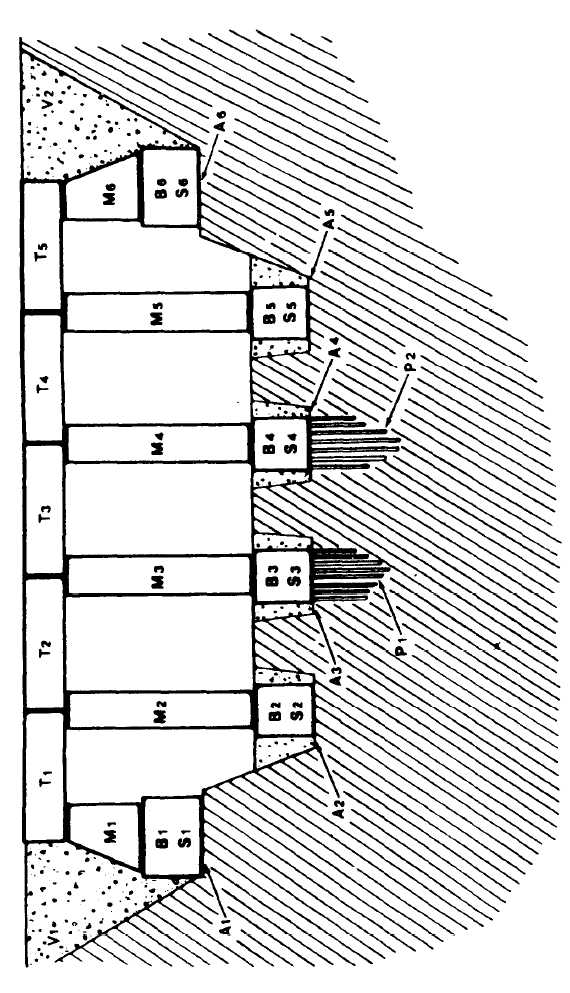
\includegraphics[width=.4\textwidth,angle=270]{images/bridgepicture}

\end{column}
\begin{column}{0.4\textwidth}
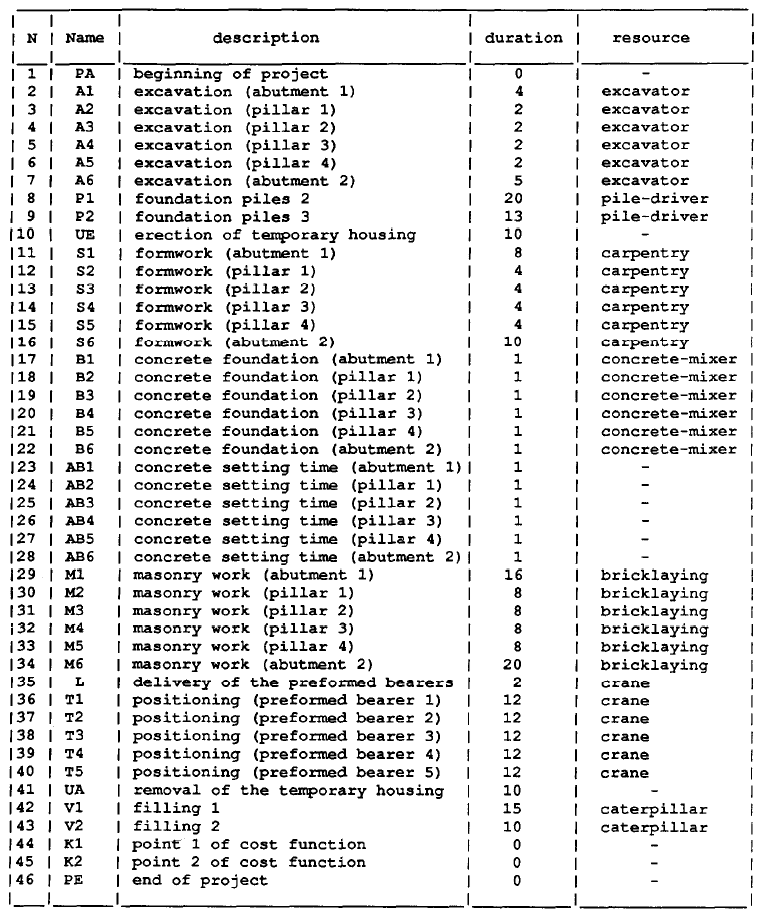
\includegraphics[width=\textwidth]{images/bridge}

%{\tiny Images from Dincbas, Simonis, Van Hentenryck. JLP 90. \cite{DincbasSH90}}
\end{column}
\end{columns}

\end{frame}

\begin{frame}
\frametitle{A Gentle Guide to Constraint Logic Programming (Niederlinski 2014~\cite{Niederlinski2014})}
\begin{columns}
\begin{column}{0.5\textwidth}
\begin{itemize}
\item Discusses many scheduling examples
\item Most are open-coded, no separation of program and data
\item ECLiPSe code given
\item Result visualizations given
\end{itemize}
\end{column}
\begin{column}{0.5\textwidth}
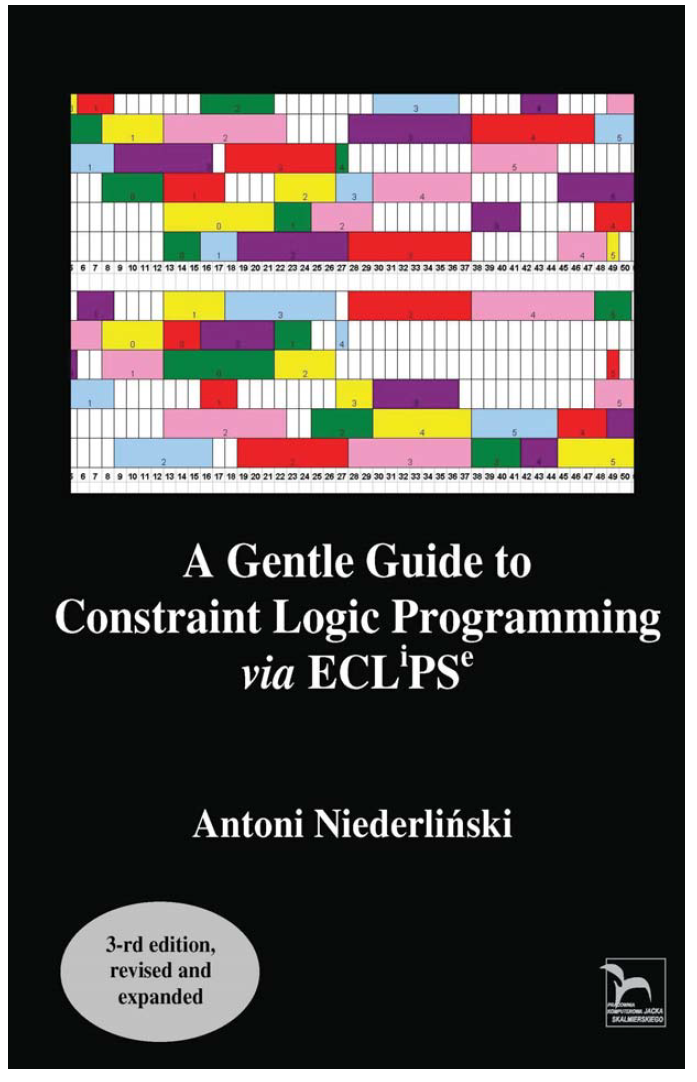
\includegraphics[width=.6\textwidth]{images/Niederlinski14titlepage}
\end{column}
\end{columns}
\end{frame}

\begin{frame}[fragile]
\frametitle{Ship Loading Example}
\begin{columns}
\begin{column}{0.5\textwidth}
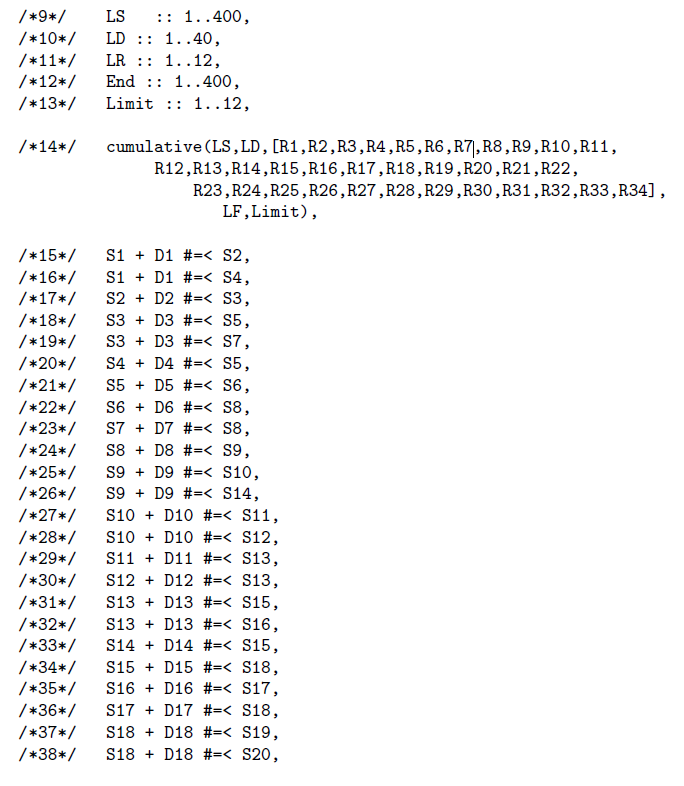
\includegraphics[width=.85\textwidth]{images/shiploadingcode}
\end{column}
\begin{column}{0.5\textwidth}
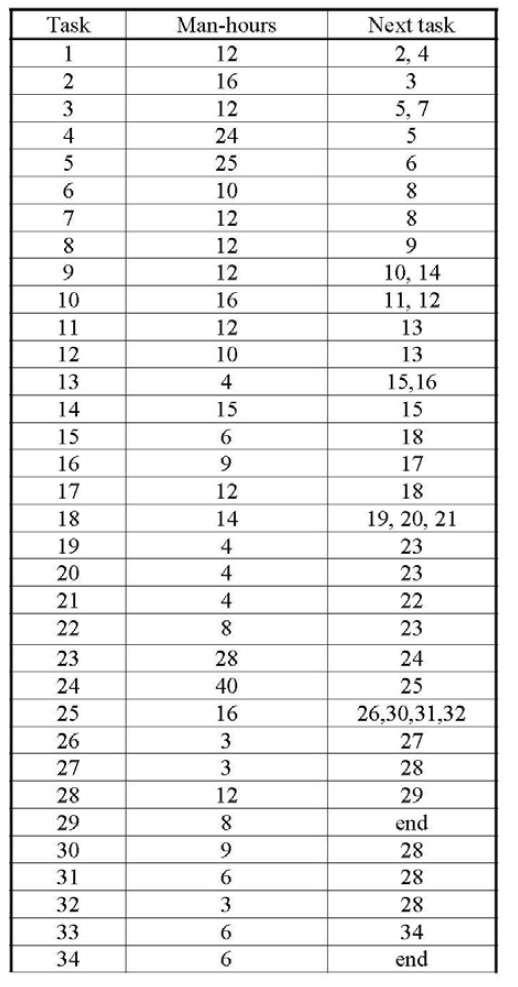
\includegraphics[width=.5\textwidth]{images/shiploading}
\end{column}
\end{columns}
\end{frame}




\begin{frame}[fragile]
\frametitle{Job-Shop (Wallace, 2020~\cite{DBLP:books/sp/Wallace20})}
\begin{columns}
\begin{column}{0.5\textwidth}
{\tiny
\begin{verbatim}
int: n_machines; 
int: n_jobs; 
int: n_tasks = n_machines; 
set of int: jobs = 1..n_jobs;
set of int: tasks = 1..n_tasks;
set of int: machines = 1..n_machines ;
array [jobs, tasks] of machines: jt_machine;
array [jobs, tasks] of int: jt_duration;
int: max_end = 1050 ;

array [jobs, tasks] of var 0.. max_end: jt_start;
var 0..max_end: t_end ;

constraint
forall ( j in jobs, k in 1..(n_tasks - 1) ) (
  jt_start[j, k] + jt_duration[j, k] <=
    jt_start[j, k + 1]
);
include "disjunctive.mzn" ;
constraint
forall(m in machines)
  (disjunctive(
    [jt_start[j,t]|j in jobs,t in tasks where jt_machine[j,t]=m],
    [jt_duration[j,t]|j in jobs, t in tasks where jt_machine[j,t]=m])
) ;

solve minimize t_end ;
\end{verbatim}
}
\end{column}
\begin{column}{0.5\textwidth}
{\tiny
\begin{verbatim}
n_jobs = 10;
n_machines = 10;
jt_machine = array2d(jobs, tasks,
[ 0, 1, 2, 3, 4, 5, 6, 7, 8, 9,
0, 2, 4, 9, 3, 1, 6, 5, 7, 8,
1, 0, 3, 2, 8, 5, 7, 6, 9, 4,
1, 2, 0, 4, 6, 8, 7, 3, 9, 5,
2, 0, 1, 5, 3, 4, 8, 7, 9, 6,
2, 1, 5, 3, 8, 9, 0, 6, 4, 7,
1, 0, 3, 2, 6, 5, 9, 8, 7, 4,
2, 0, 1, 5, 4, 6, 8, 9, 7, 3,
0, 1, 3, 5, 2, 9, 6, 7, 4, 8,
1, 0, 2, 6, 8, 9, 5, 3, 4, 7 ]);
jt_duration = array2d(jobs, tasks, [
29, 78, 9, 36, 49, 11, 62, 56, 44, 21,
43, 90, 75, 11, 69, 28, 46, 46, 72, 30,
91, 85, 39, 74, 90, 10, 12, 89, 45, 33,
81, 95, 71, 99, 9, 52, 85, 98, 22, 43,
14, 6, 22, 61, 26, 69, 21, 49, 72, 53,
84, 2, 52, 95, 48, 72, 47, 65, 6, 25,
46, 37, 61, 13, 32, 21, 32, 89, 30, 55,
31, 86, 46, 74, 32, 88, 19, 48, 36, 79,
76, 69, 76, 51, 85, 11, 40, 89, 26, 74,
85, 13, 61, 7, 64, 76, 47, 52, 90, 45
]);
\end{verbatim}
}
\end{column}
\end{columns}
\end{frame}

\begin{frame}
\frametitle{Resource-Constrained Project Scheduling Problem (RCPSP) (Bourreau et al., 2019~\cite{Bourreau2019})}
\begin{columns}
\begin{column}{0.5\textwidth}
\begin{itemize}
\item RCPSP with different approaches
\item Different solvers, Choco-Solver, OPL Studio
\item Complete Java projects
\item Focus on modelling alternatives, performance
\item Partial search (LDS)
\item Also considers job-shop
\end{itemize}
\end{column}
\begin{column}{0.5\textwidth}
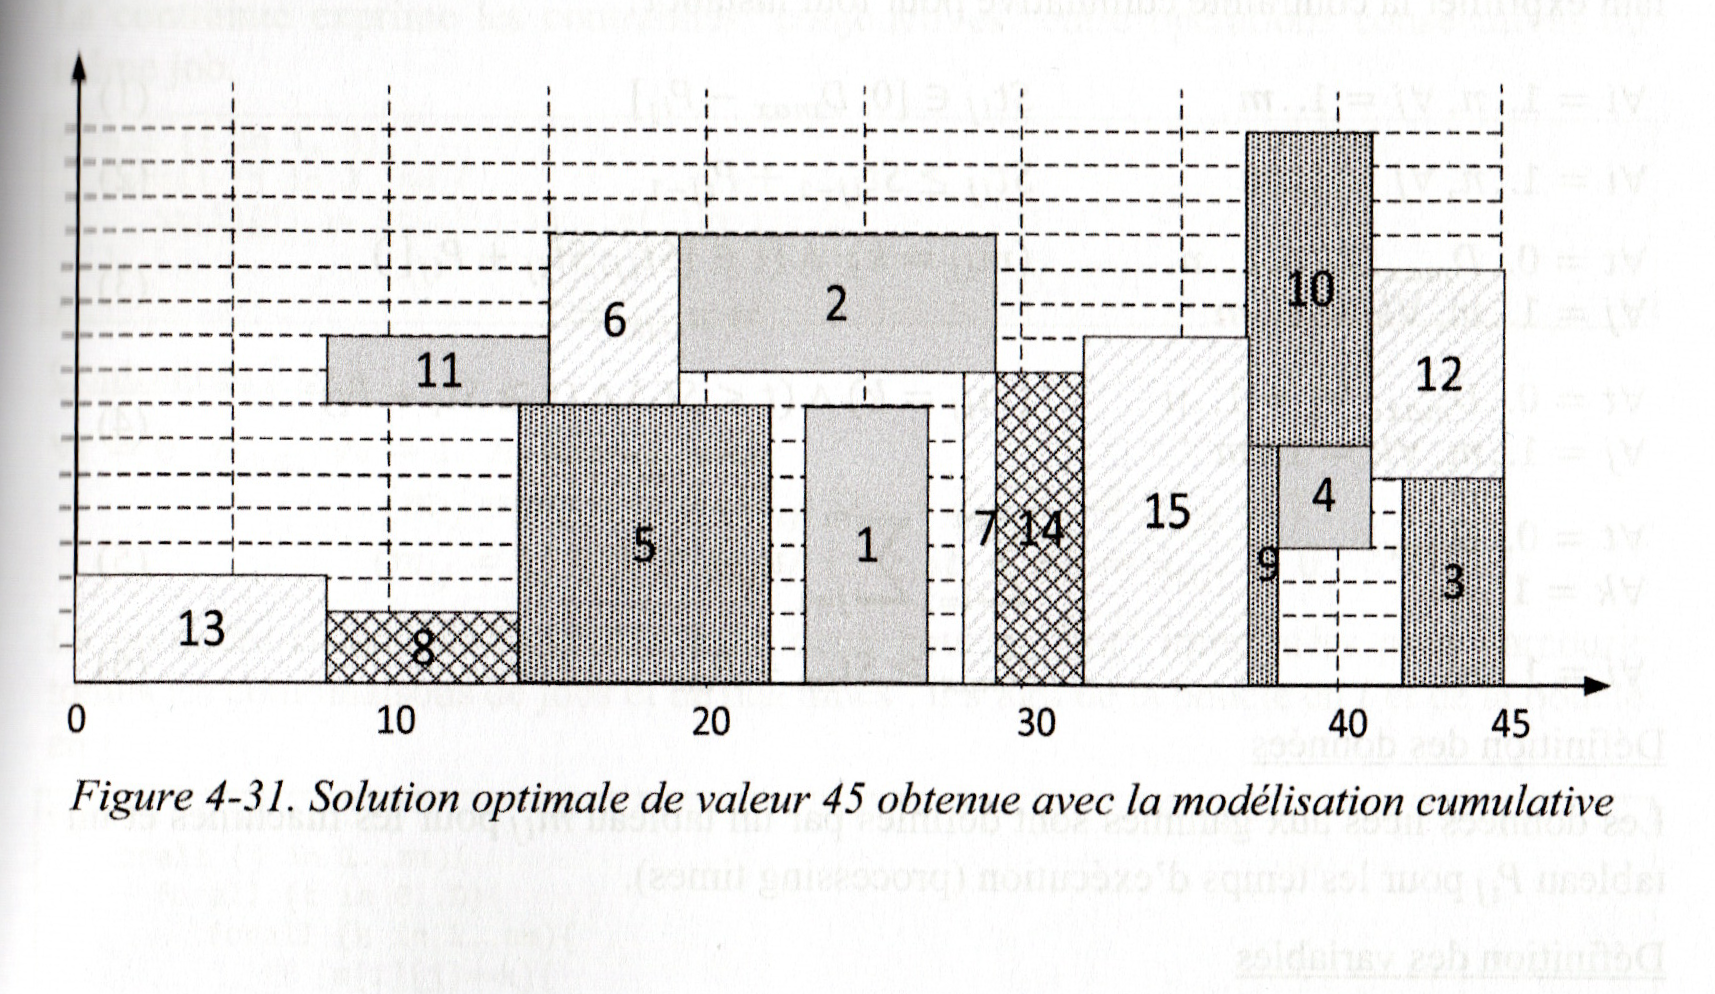
\includegraphics[width=\textwidth]{images/rcpspgantt}
\end{column}
\end{columns}
\end{frame}

\begin{frame}
\frametitle{Common Points}
\begin{itemize}
\item A good number of scheduling problems are presented
\item Often not in a form that allows Constraint Acquisition to work
\item Needs a lot of work to present data and solutions in machine readable form
\item Resulting models are easy for tools to find, even with single (few) positive examples
\end{itemize}
\end{frame}



\section{CP Based Scheduling Literature}

\subsection{Literature Survey}

\begin{frame}
\frametitle{Motivation}
\begin{itemize}
\item More and more papers attach data
\item But, every paper uses different format
\item CA ideally should be able to deal with these
\item Broad basis for requirements analysis
\item Most papers do not make it easy to understand data
\end{itemize}
\end{frame}

\begin{frame}
\frametitle{Methodology}
\begin{itemize}
\item Use DBLP as primary source
\item Extract relevant meta-data
\item Text analysis of pdf to find shared concepts
\item Manual extraction of some features
\end{itemize}
\end{frame}

\begin{frame}
\frametitle{Existing Literature Surveys}
\begin{itemize}
\item Optimal methods for resource allocation and scheduling: a cross-disciplinary survey. Lombardi, Milano. 2012~\cite{LombardiM12}.
\begin{itemize}
\item Compares CP, MIP and hybrid methods
\item Gives examples of models and solution methods
\item From 2012, a lot of progress since then
\end{itemize}
\item Applications of constraint programming in production scheduling problems: A descriptive bibliometric analysis. Prata, Abreu, and Nagano. 2024~ \cite{PrataAN23}.
\begin{itemize}
\item Deeply flawed paper: data, methodology and analysis
\item Only focuses on flow/job/open shop
\end{itemize}
\end{itemize}
\end{frame}



\begin{frame}
\frametitle{Literature Survey - Recent Articles}
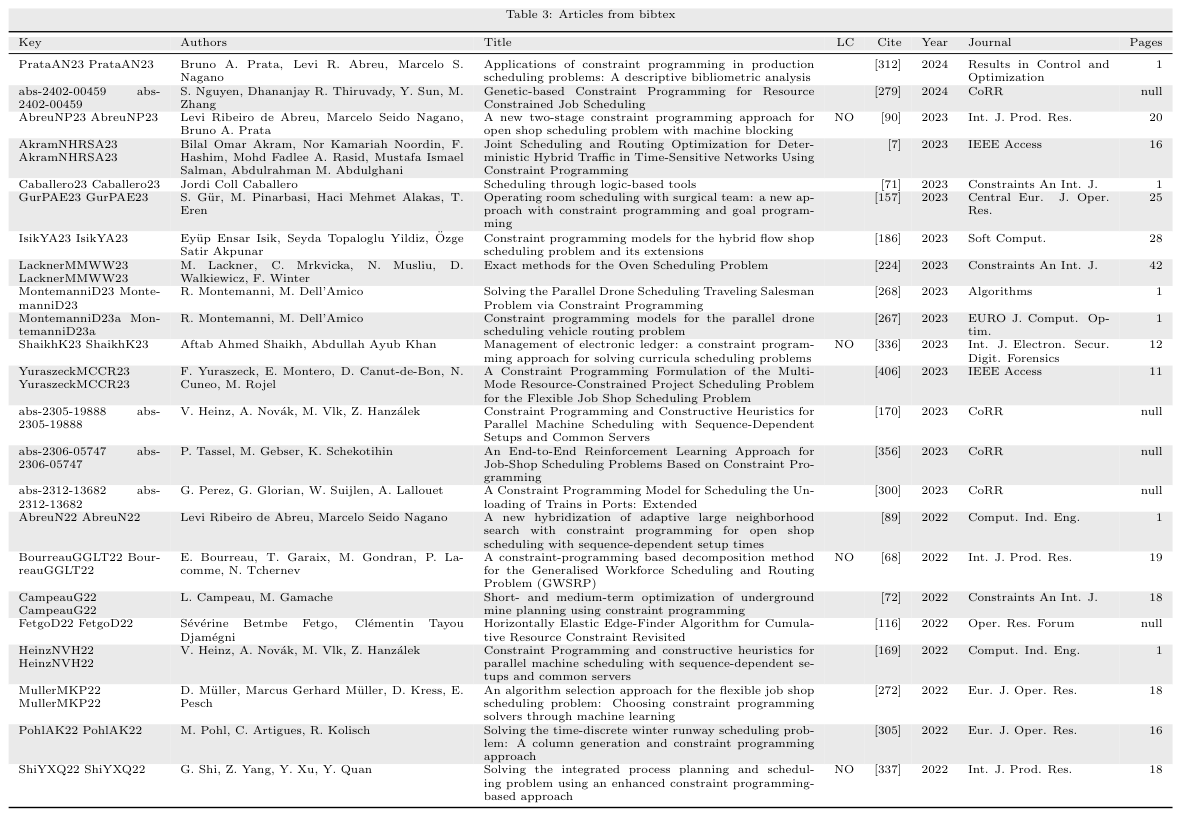
\includegraphics[width=\textwidth]{images/articles1}
\end{frame}

\begin{frame}
\frametitle{Literature Survey - Extracted Concepts}
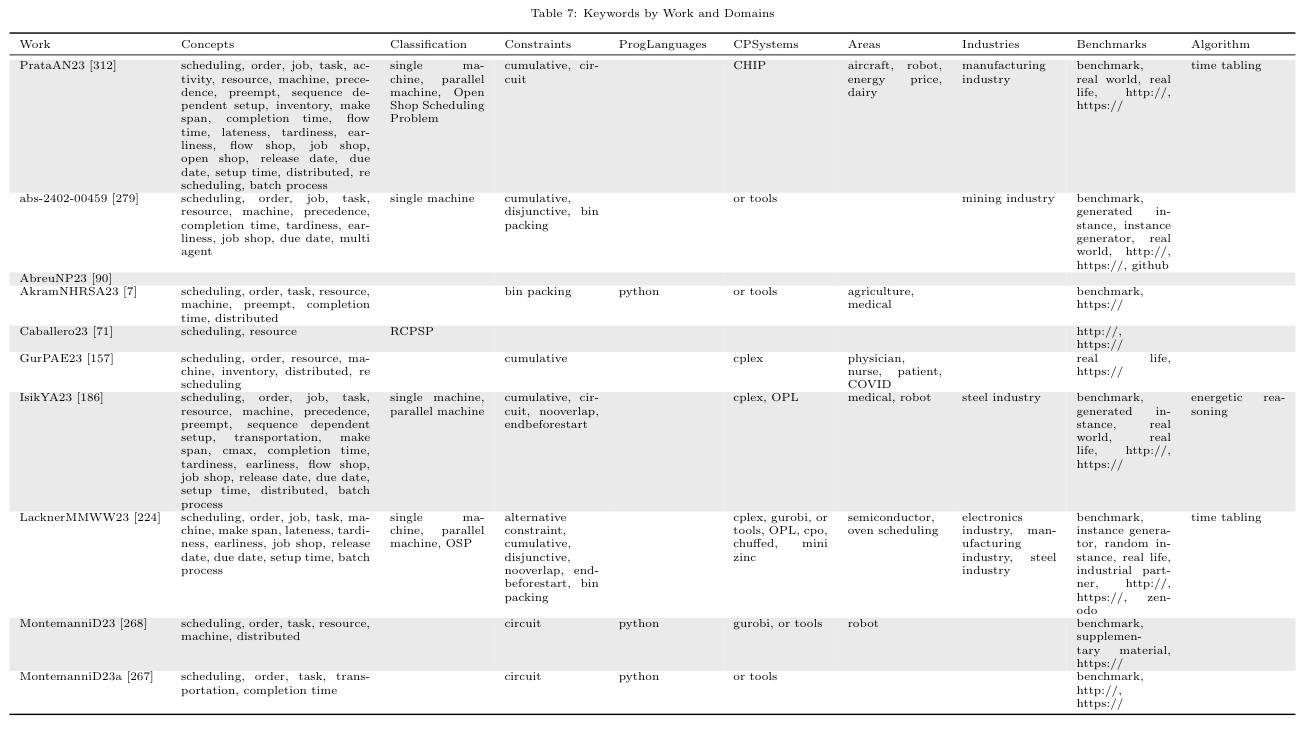
\includegraphics[width=.95\textwidth]{images/concepts}
\end{frame}


\begin{frame}
\frametitle{Literature Survey - Supplementary Materials}
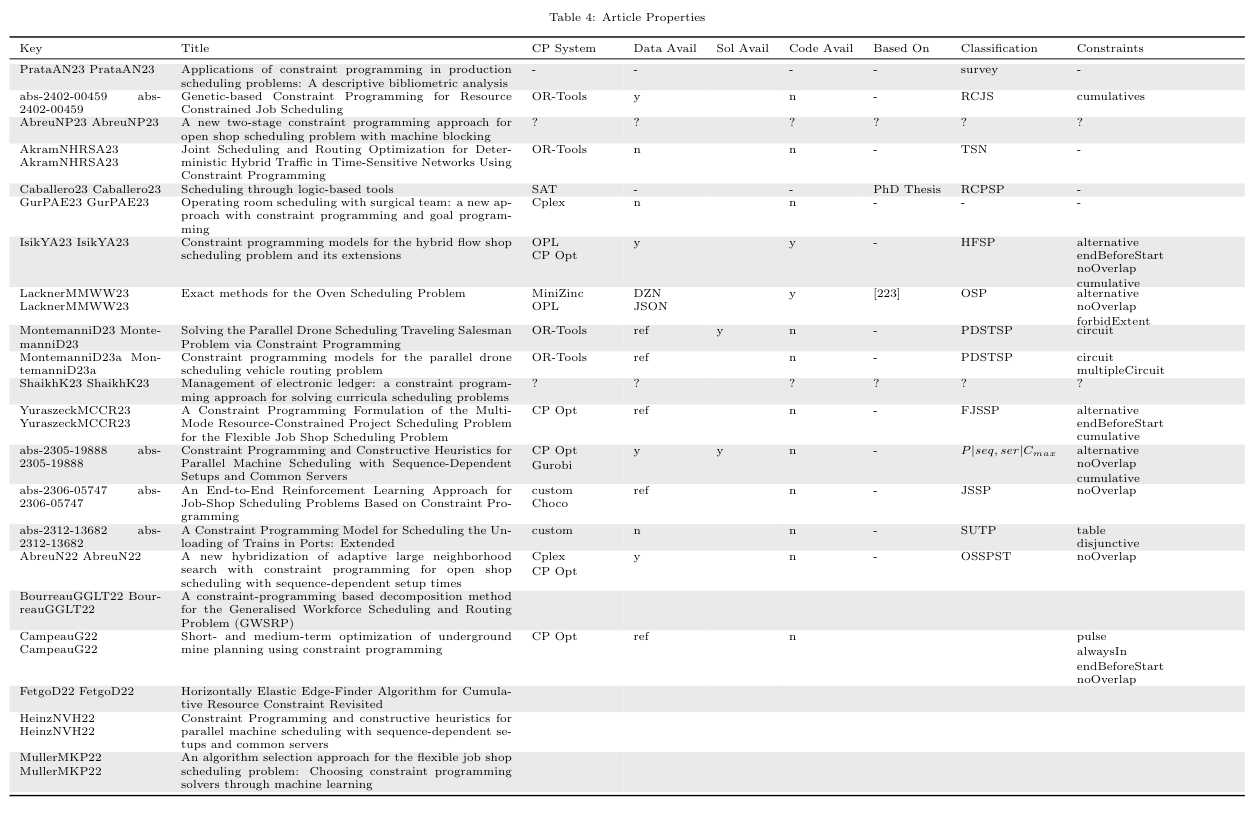
\includegraphics[width=\textwidth]{images/articles2}
\end{frame}

\begin{frame}
\frametitle{Literature Survey - The same for Papers}
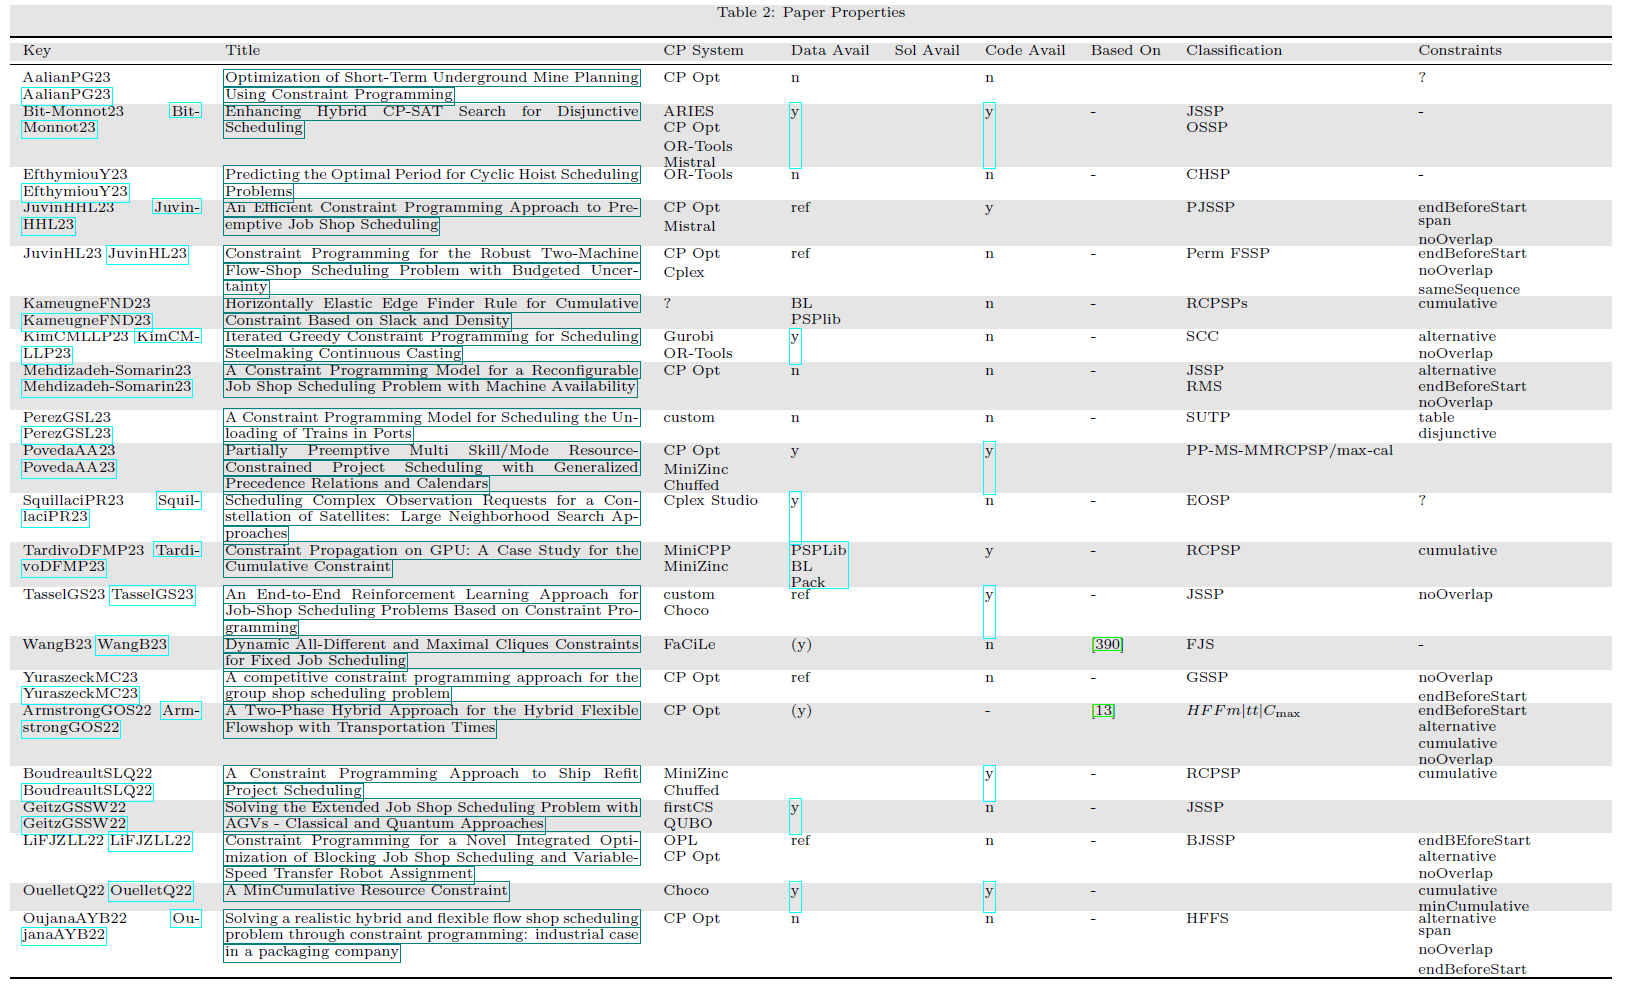
\includegraphics[width=\textwidth]{images/papers2}
\end{frame}

\begin{frame}
\frametitle{Literature Survey - Application Areas}
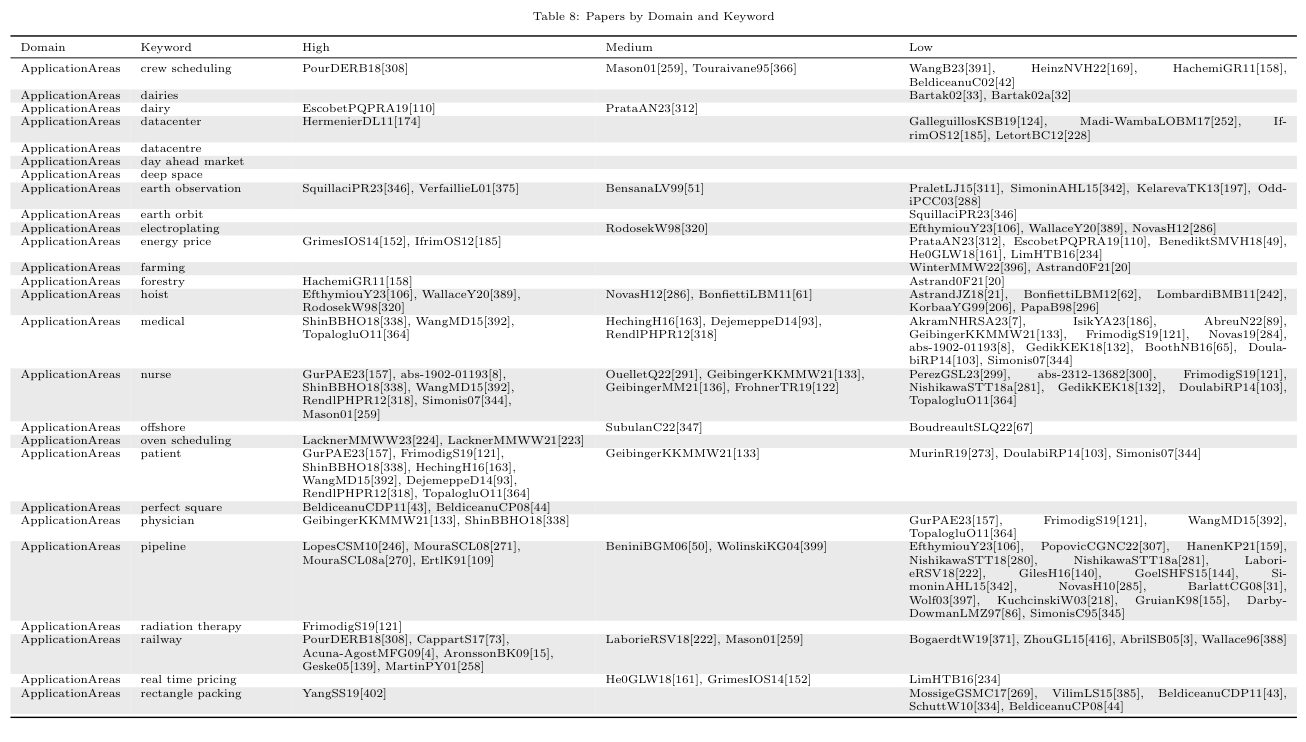
\includegraphics[width=.9\textwidth]{images/applicationareas}
\end{frame}

\begin{frame}
\frametitle{Literature Survey - Frequent Authors}
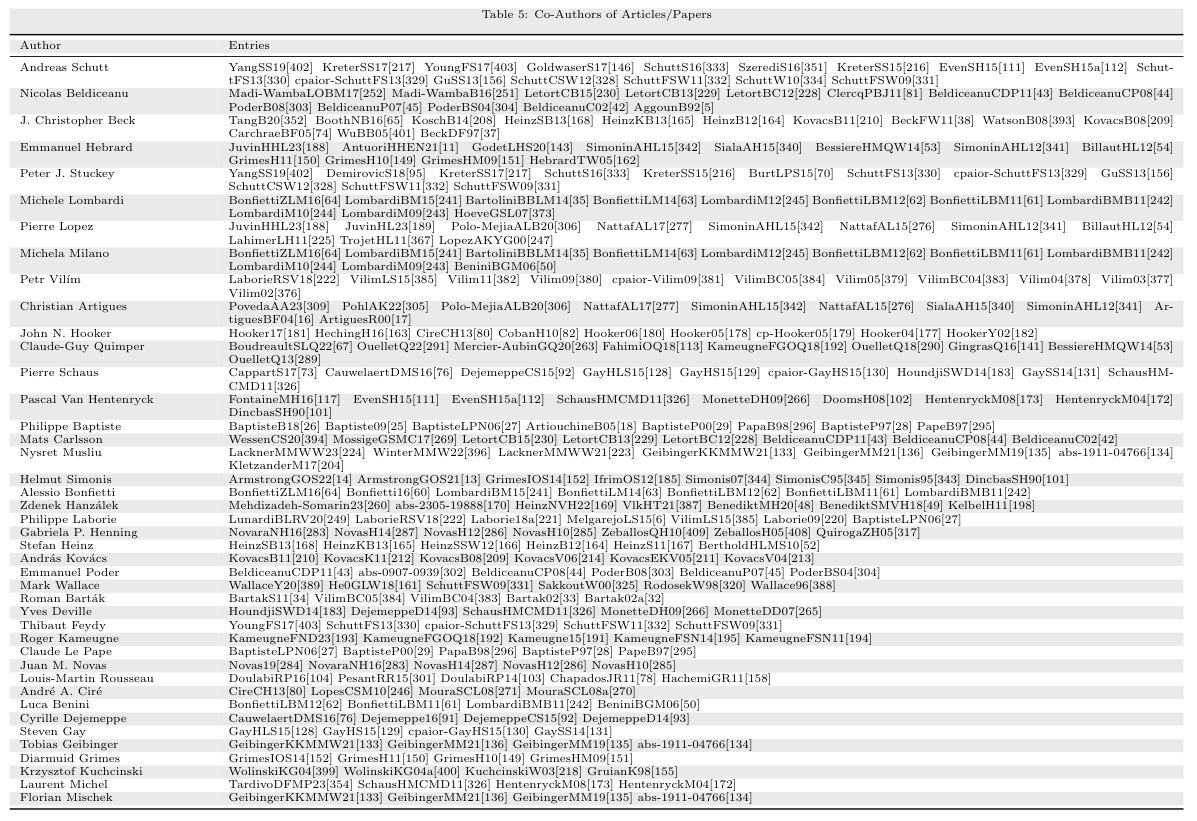
\includegraphics[width=.74\textwidth]{images/authors}
\end{frame}




\subsection{Papers with Data and (Solutions or Programs)}

\begin{frame}
\frametitle{Most Recent Papers/Articles with Supplementary Materials}

{\scriptsize
\begin{tabular}{lrrllll} \toprule
Key & Size & Instances & MetaData & Format & Solutions & Checker \\ \midrule
AbreuN22 \cite{AbreuN22} & 1.3MB & 192 & n & TS & n & n\\
AntuoriHHEN21 \cite{AntuoriHHEN21}& 23.3MB& 120 & n & TS & n & n\\
ArmstrongGOS21 \cite{ArmstrongGOS21}& 11MB & 225 & n & dzn & n & n\\
BenderWS21 \cite{BenderWS21}& 116KB& 84 & y & TS & n & n\\
Bit-Monnot23 \cite{Bit-Monnot23}& 23.5MB & 357 & n & TS & n & n\\
GeibingerKKMMW21 \cite{GeibingerKKMMW21}& 40KB& & & & & n\\
GeibingerMM21 \cite{GeibingerMM21}& 13.9MB & & & & & n\\
GeitzGSSW22 \cite{GeitzGSSW22}& 16.0KB & & & & & n\\
IsikYA23 \cite{IsikYA23} & 3.9MB & & & & & n\\
KimCMLLP23 \cite{KimCMLLP23}& 4.1MB & & & & & n\\
KovacsTKSG21 \cite{KovacsTKSG21}& 138MB & 18 & n & JSON & n & n\\
\bottomrule
\end{tabular}
}

\end{frame}


\subsection{Format Examples}

\begin{frame}
\frametitle{AbreuN22 \cite{AbreuN22}}
\begin{columns}
\begin{column}{0.5\textwidth}
\begin{itemize}
\item
\end{itemize}
\end{column}
\begin{column}{0.5\textwidth}
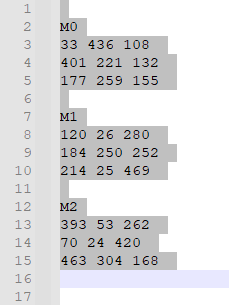
\includegraphics[width=.5\textwidth]{images/AbreuN22}
\end{column}
\end{columns}
\end{frame}

\begin{frame}
\frametitle{AntuoriHHEN21 \cite{AntuoriHHEN21}}
\begin{columns}
\begin{column}{0.5\textwidth}
\begin{itemize}
\item
\end{itemize}
\end{column}
\begin{column}{0.5\textwidth}
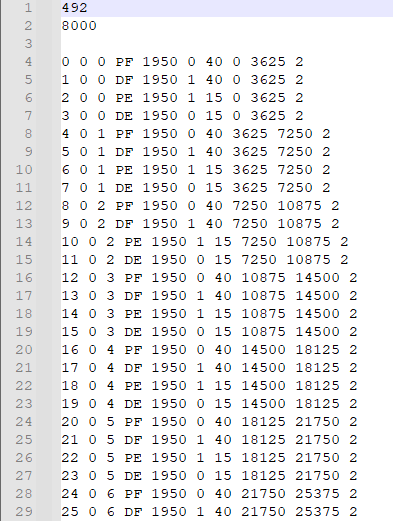
\includegraphics[width=.8\textwidth]{images/AntuoriHHEN21}
\end{column}
\end{columns}
\end{frame}


\begin{frame}
\frametitle{ArmstrongGOS21~\cite{ArmstrongGOS21}}
\begin{columns}
\begin{column}{0.5\textwidth}
\begin{itemize}
\item Instances in MiniZinc .dzn format
\item Single file per instance
\item Matches program in paper
\item Integers, String, Arrays, Sets
\item Tedious to parse for other solvers
\item Could now be replaced by JSON
\item Checker is easy to add
\end{itemize}
\end{column}
\begin{column}{0.5\textwidth}
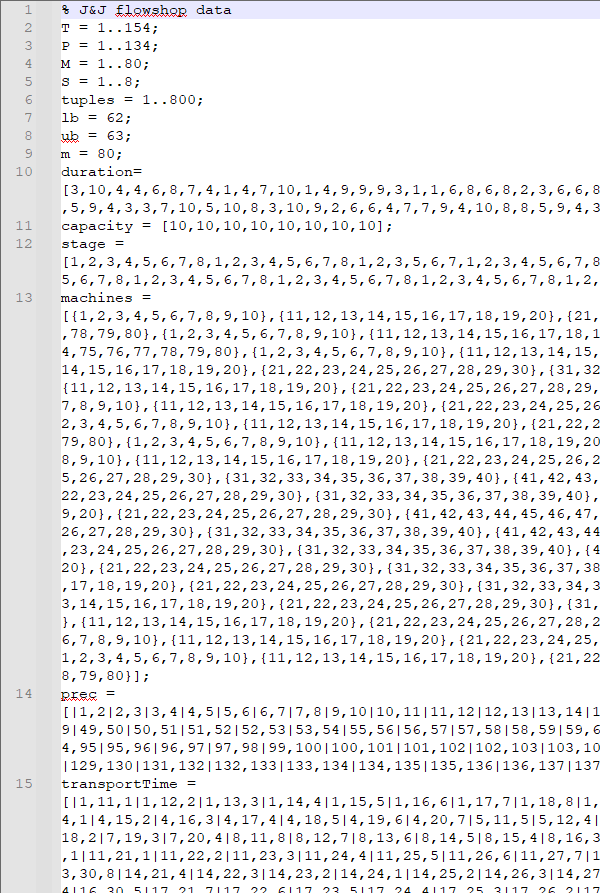
\includegraphics[width=.7\textwidth]{images/ArmstrongGOS21}
\end{column}
\end{columns}
\end{frame}

\begin{frame}
\frametitle{BenderWS21 \cite{BenderWS21}}
\begin{columns}
\begin{column}{0.5\textwidth}
\begin{itemize}
\item Describes format of data
\end{itemize}
\end{column}
\begin{column}{0.5\textwidth}
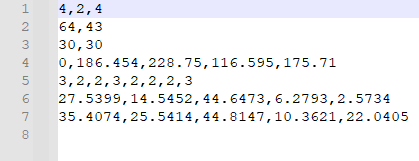
\includegraphics[width=\textwidth]{images/BenderWS21}
\end{column}
\end{columns}
\end{frame}

\begin{frame}
\frametitle{Bit-Monnot23 \cite{Bit-Monnot23}}
\begin{columns}
\begin{column}{0.5\textwidth}
\begin{itemize}
\item Mix of strings and numbers
\item Text stream
\item Different formats for job shop and open shop instances
\end{itemize}
\end{column}
\begin{column}{0.5\textwidth}
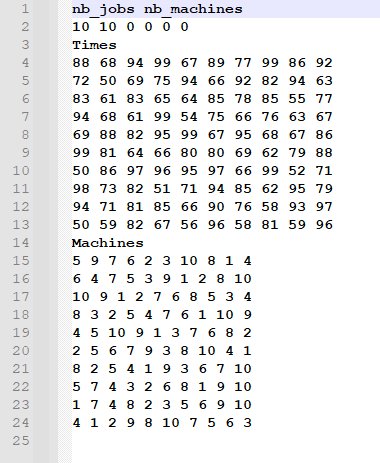
\includegraphics[width=.7\textwidth]{images/Bit-Monnot23}
\end{column}
\end{columns}
\end{frame}


\begin{frame}
\frametitle{KovacsTKSG21~\cite{KovacsTKSG21}}
\begin{columns}
\begin{column}{0.5\textwidth}
\begin{itemize}
\item Nice JSON format of data
\item Real-life data
\item One instance per file, one file per instance
\item Task length given as float
\item Machine capacity given as float
\end{itemize}
\end{column}
\begin{column}{0.5\textwidth}
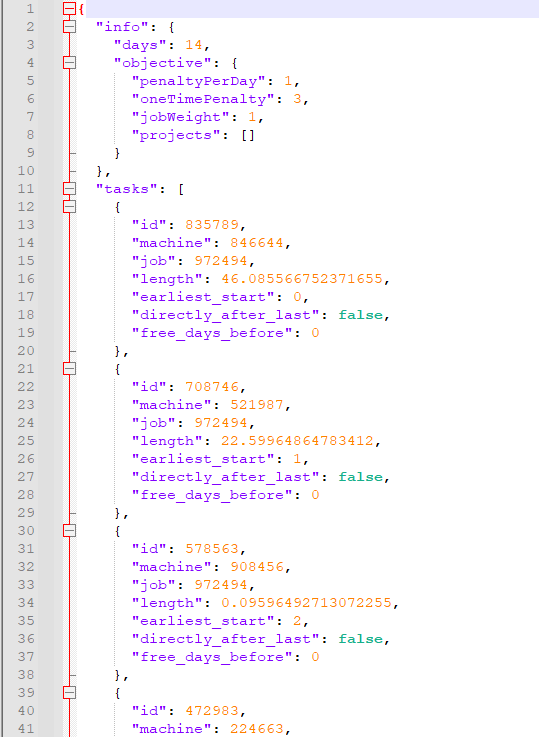
\includegraphics[width=\textwidth]{images/KovacsTKSG21}
\end{column}
\end{columns}
\end{frame}

\begin{frame}
\frametitle{Challenges}
\begin{itemize}
\item Data formats are often ad-hoc, token streams common
\item Meaning of value depends on position in stream
\item Solutions very rarely provided
\begin{itemize}
\item If given, only one (best) solution is given
\item Sometimes can be generated from code which is provided
\end{itemize}
\item Checkers non-existent
\item For many papers, extracting the constraint model is not the challenge
\begin{itemize}
\item Finding a good solution quickly enough is
\end{itemize} 
\end{itemize}
\end{frame}



\section{Realistic Examples}

\begin{frame}
\frametitle{Realistic Examples}
\begin{itemize}
\item Two examples of a more complex nature
\item Realistic, but not real problem set
\item Show complexity of real-world problems 
\end{itemize}
\end{frame}


\subsection{ROADEF2022}

\begin{frame}
\frametitle{Roadef2022 Challenge}
\begin{columns}
\begin{column}{0.5\textwidth}
\begin{itemize}
\item Competition by French OR society Roadef, European OR society Euro 
\item Problem provided by Renault
\item Schedule transport of components from suppliers to factories
\item Decide when to transport item, how to pack them into trucks
\item Decide how many resources (trucks) are needed
\item Not a vehicle routing problem (routes predefined and given)
\item Objective Minimize cost (resources plus earliness cost of items)
\end{itemize}
\end{column}
\begin{column}{0.5\textwidth}
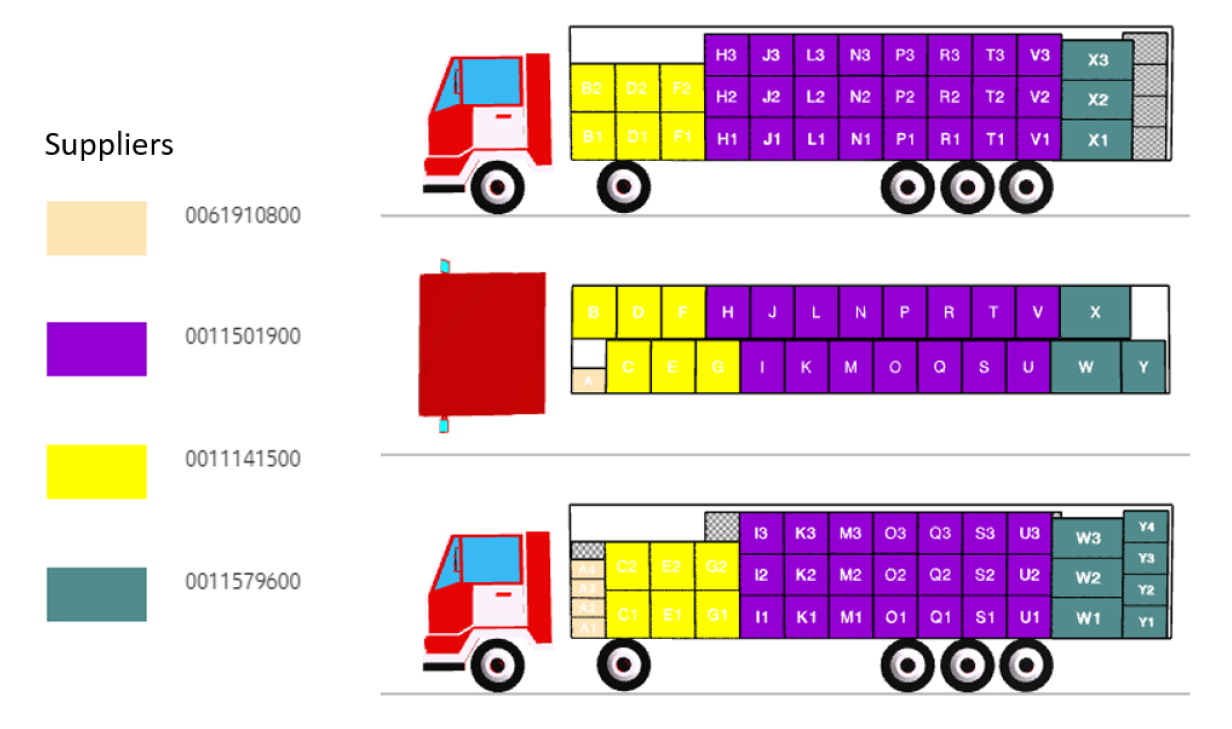
\includegraphics[width=\textwidth]{images/roadefsuppliers}
\end{column}
\end{columns}
\end{frame}

\begin{frame}
\frametitle{Input Data}
Potential Trucks

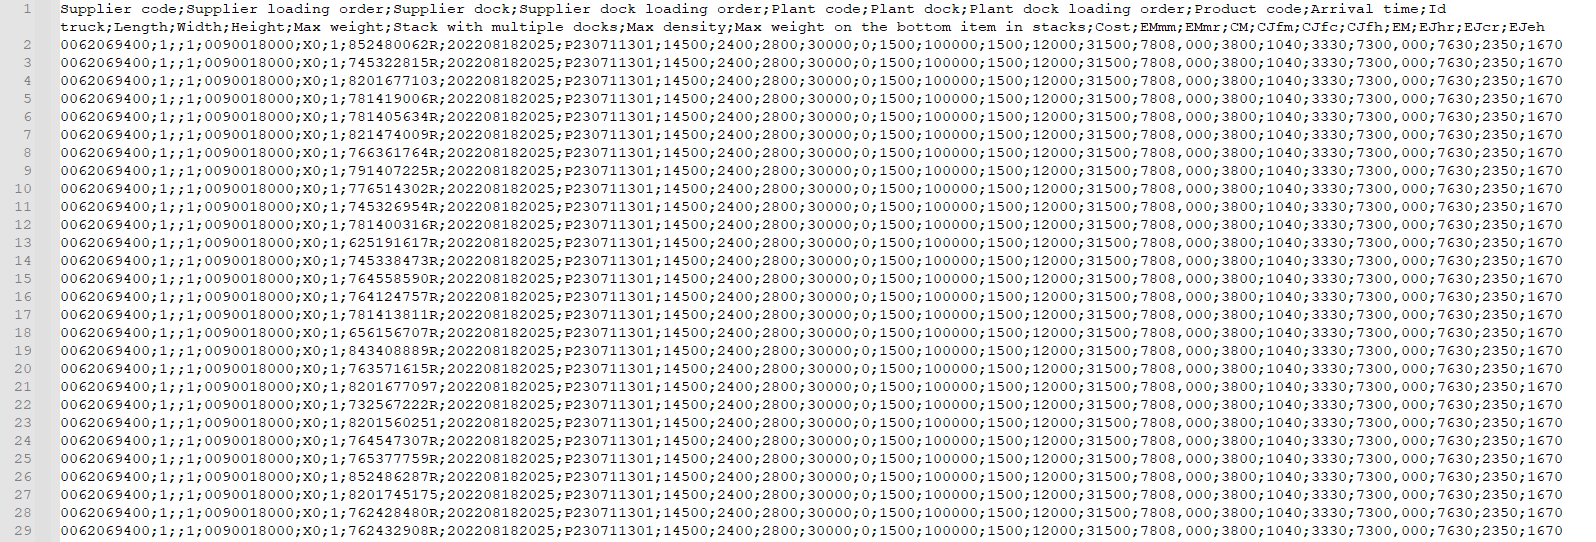
\includegraphics[width=\textwidth]{images/roadeftrucks}

\end{frame}

\begin{frame}
\frametitle{Input Data (II)}

Items to be Transported

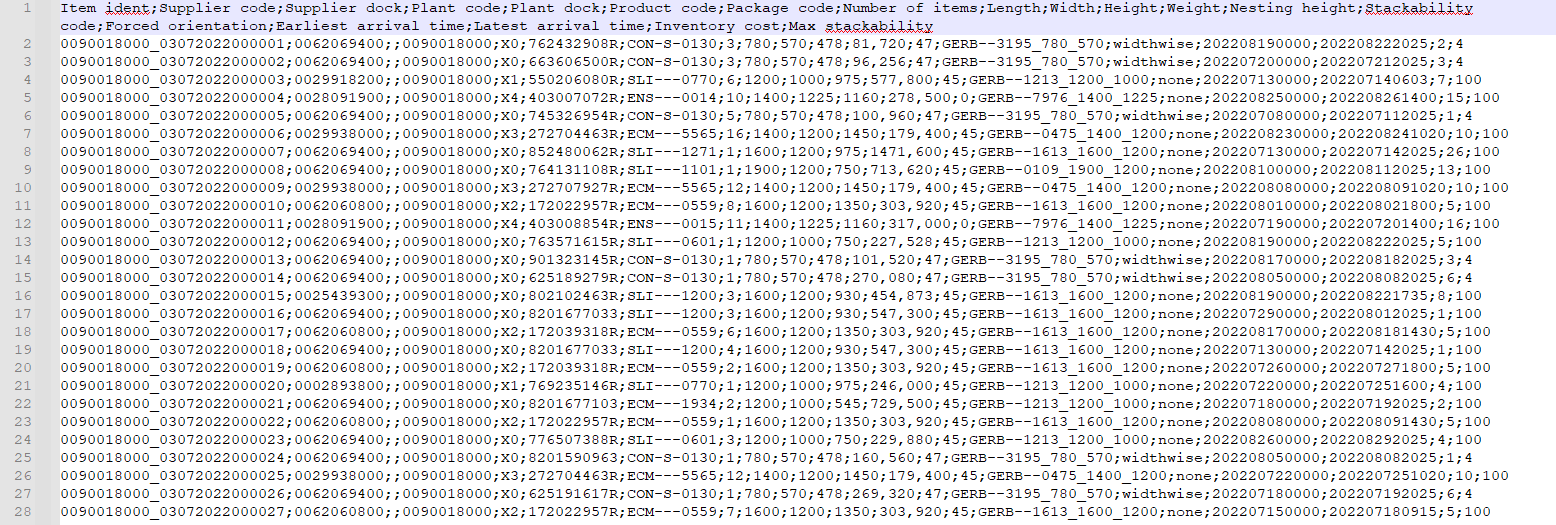
\includegraphics[width=\textwidth]{images/roadefitems}

Parameters of Problem

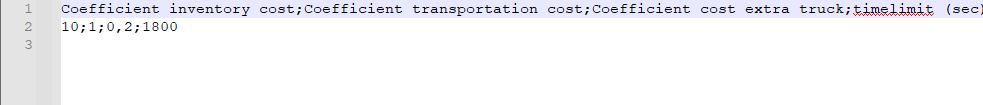
\includegraphics[width=.7\textwidth]{images/roadefparameters}
\end{frame}

\begin{frame}
\frametitle{Observations}
\begin{itemize}
\item Data size varies between instances, but is typically (very) large
\item Four stages of data availability, 150 instances in total
\item One sample solution given
\item But: Checker (in java) provided, normative
\item Problem description 11+8 pages
\item Data tables not normalized, contains much redundant information
\item Normalizing data leads to UML Object Model on next slide
\end{itemize}
\end{frame}


\begin{frame}
\frametitle{Resulting Object Model}
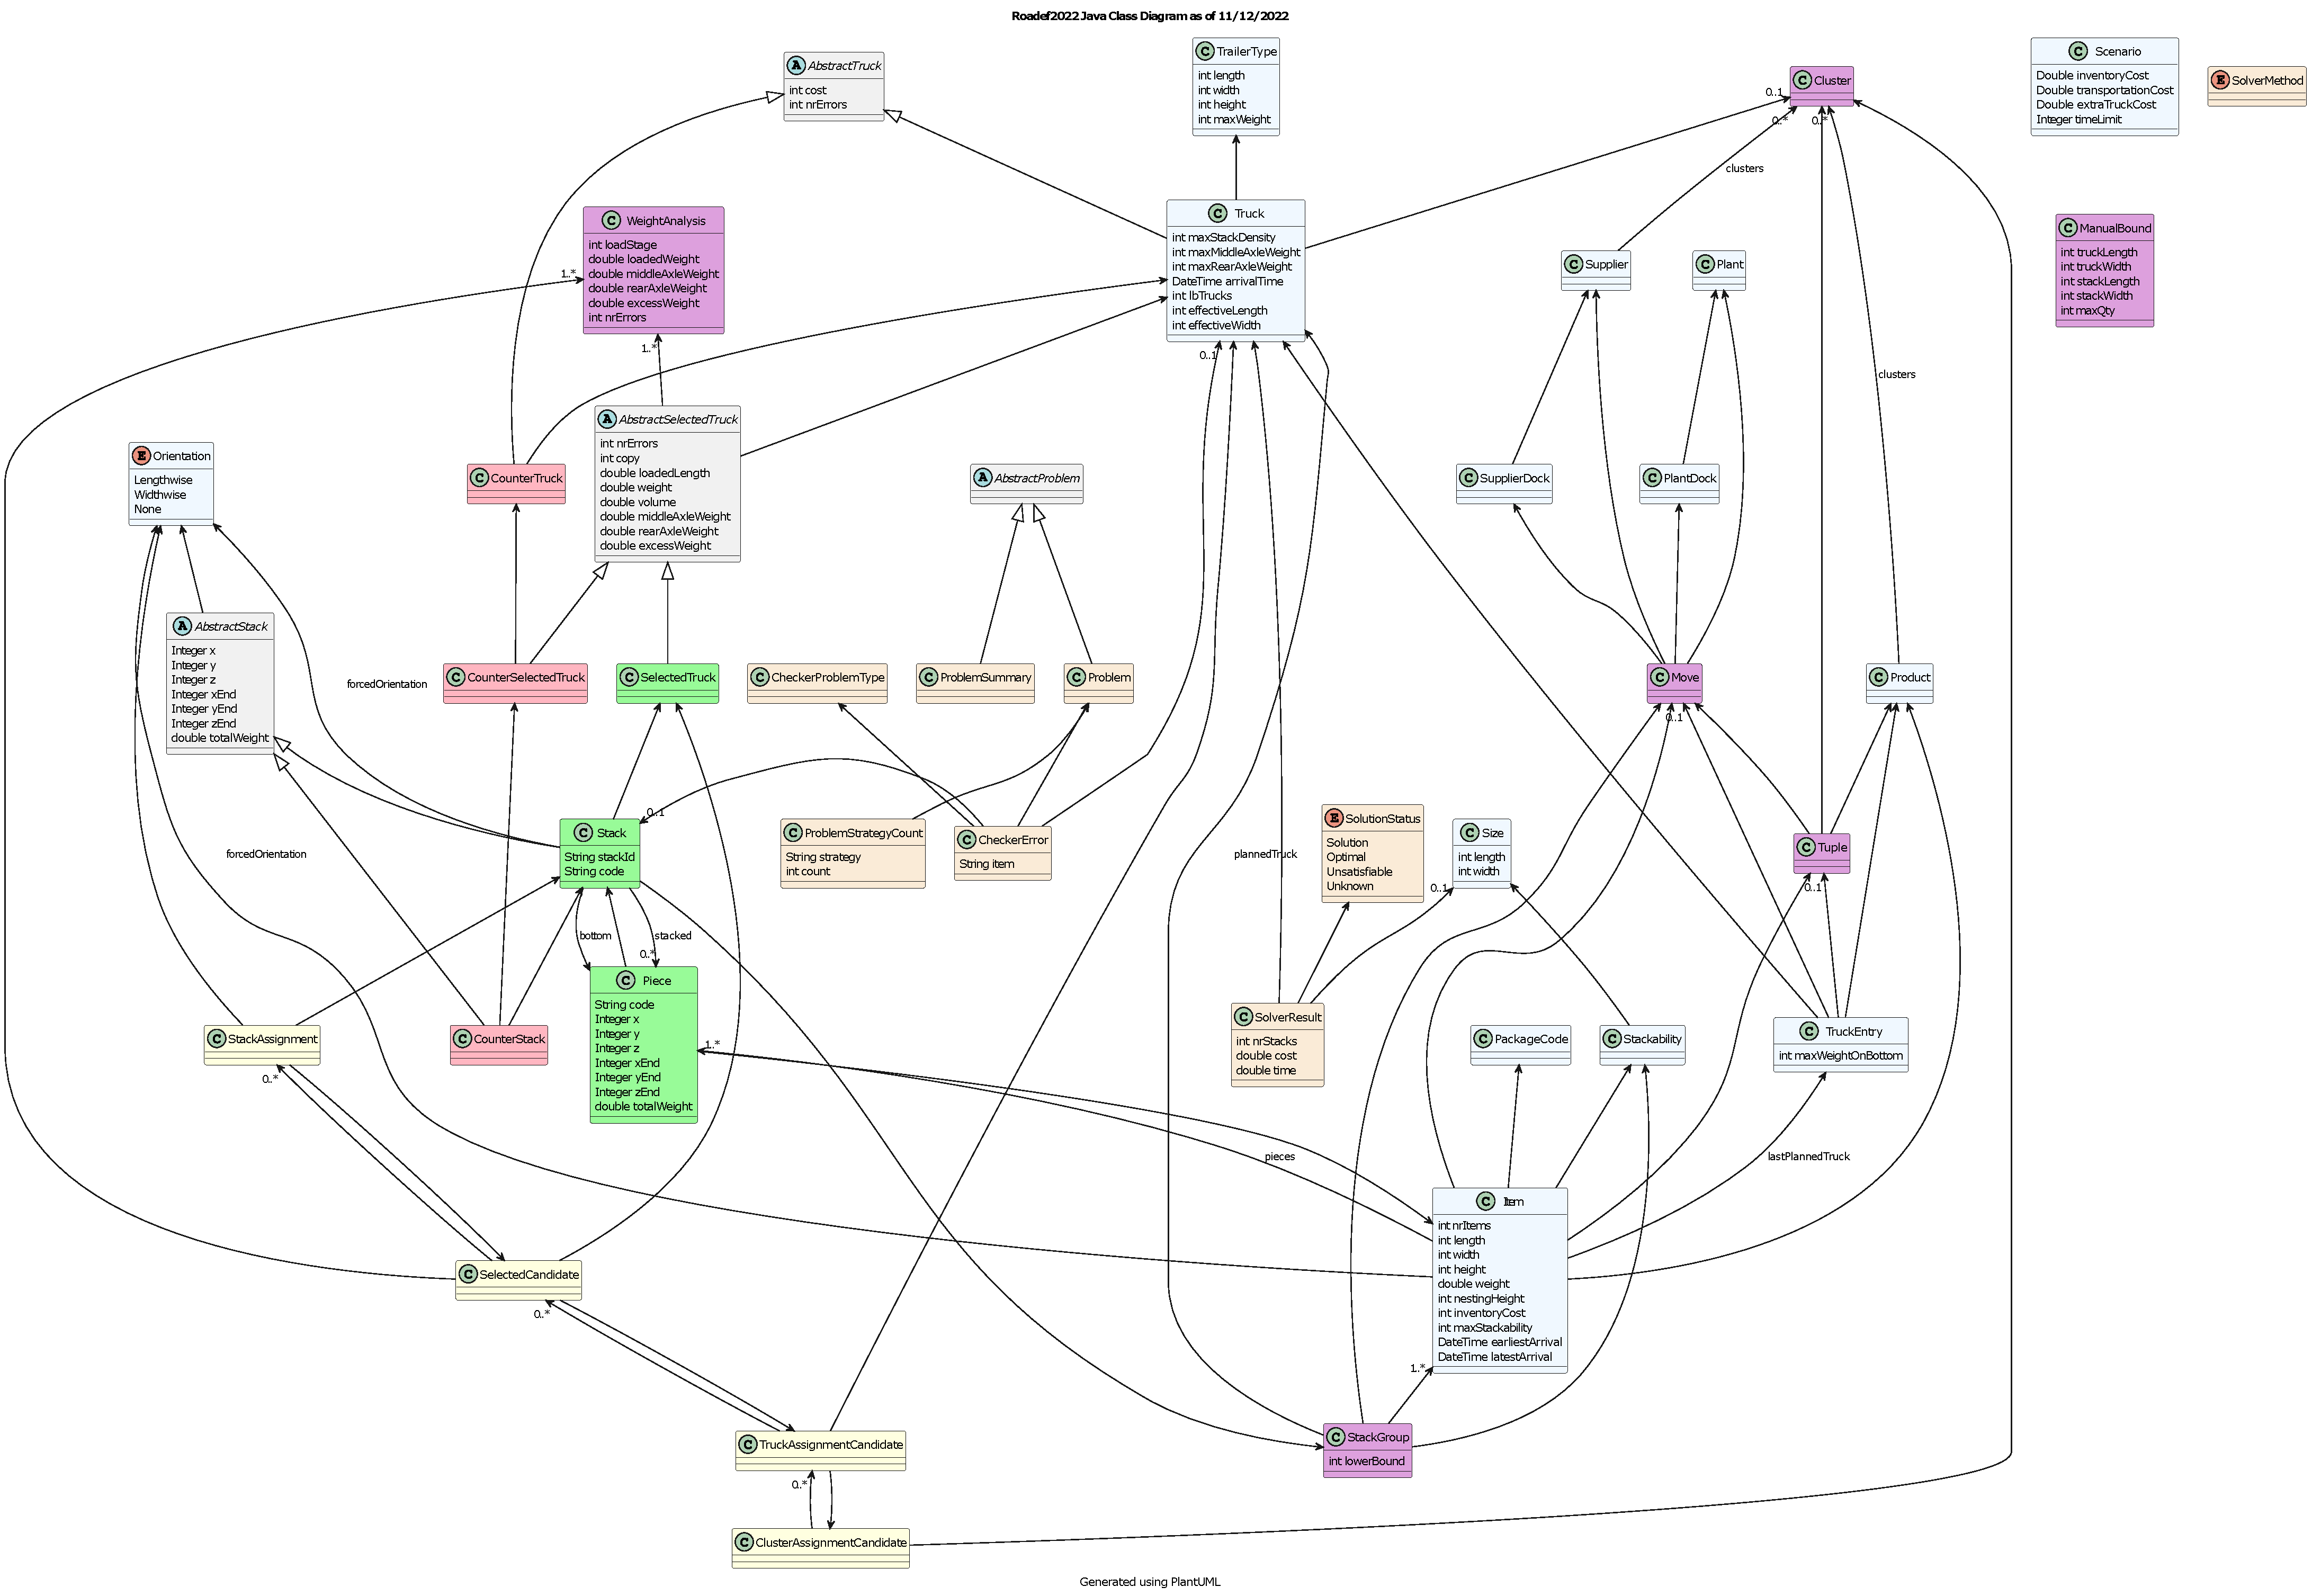
\includegraphics[width=.7\textwidth]{images/roadefuml}
\end{frame}


\begin{frame}
\frametitle{Defined Output Format}
\begin{columns}
\begin{column}{0.5\textwidth}
\begin{itemize}
\item Three files
\begin{itemize}
\item Trucks used
\item Stacks built
\item Pieces placed
\end{itemize}
\item No direct link between planned and scheduled trucks
\item Concept of stack is redundant
\item One item results in multiple pieces
\item Link between trucks, stacks, pieces and input data by string ids
\end{itemize}
\end{column}
\begin{column}{0.5\textwidth}
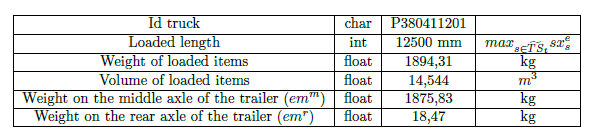
\includegraphics[width=\textwidth]{images/roadefresulttrucks}
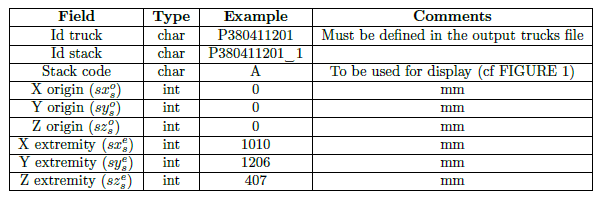
\includegraphics[width=\textwidth]{images/roadefresultstacks}
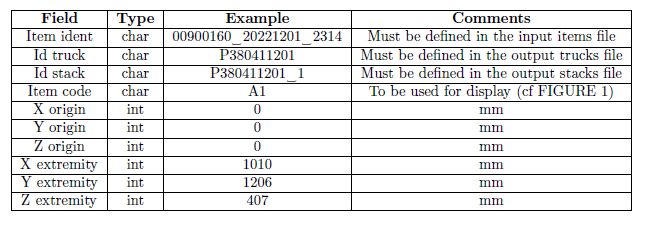
\includegraphics[width=\textwidth]{images/roadefresultitems}
\end{column}
\end{columns}
\end{frame}

\begin{frame}
\frametitle{Complex Side Constraints}
\begin{columns}
\begin{column}{0.5\textwidth}
\begin{itemize}
\item Some of the constraints are not just simple, linear formulas
\end{itemize}
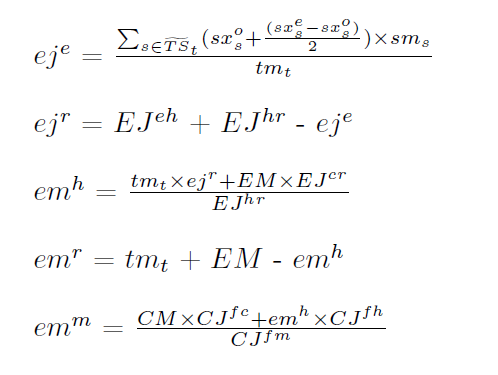
\includegraphics[width=\textwidth]{images/roadefaxleweightconstraints}
\end{column}
\begin{column}{0.5\textwidth}
\begin{itemize}
\item Interpretation requires detailed physical model
\end{itemize}
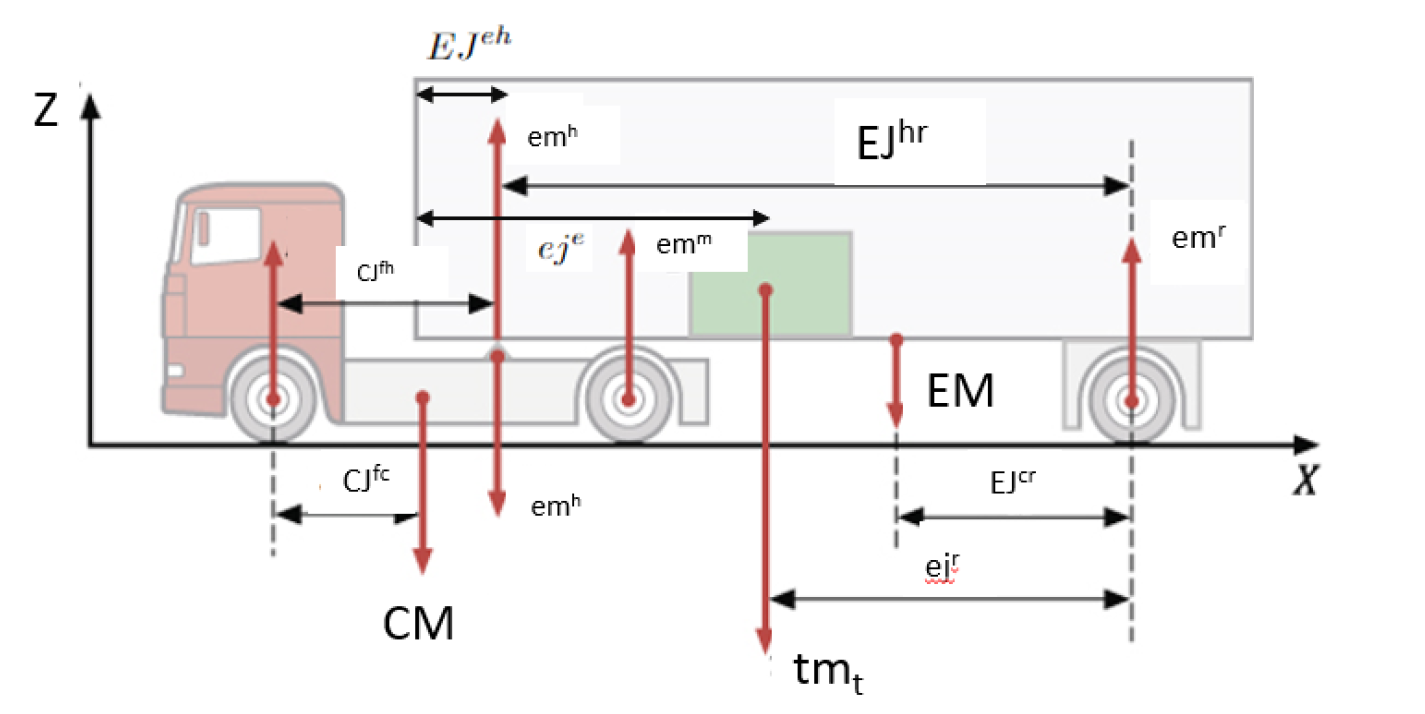
\includegraphics[width=\textwidth]{images/roadeftrailerfields}
\end{column}
\end{columns}
\end{frame}


\begin{frame}
\frametitle{A Grand Challenge for Constraint Acquisition}
\begin{itemize}
\item Can you extract a transferable model of this problem?
\begin{itemize}
\item Given the data and solutions of all problem instances
\end{itemize}
\item Not too hard to find packing constraints for pieces
\item Packing constraints for stacks are simple
\item Real problem
\begin{itemize}
\item How many stacks are needed?
\item How many trucks are needed?
\item Many non-trivial side constraints!
\end{itemize}
\item Previous competitions provide similar challenges
\begin{itemize}
\item There is a checker!
\item Lots of instances
\item Solutions not known until challenge end
\end{itemize}

\end{itemize}
\end{frame}





\subsection{ASSISTANT SE Use Case}

\begin{frame}
\frametitle{An Industrial Example}
\begin{itemize}
\item ASSISTANT Siemens Energy use case
\item Mid/Long-term scheduling/production planning
\item Realistic/not real data
\item Rather complex constraint model
\begin{itemize}
\item Multi-stage BOM
\item Alternative Process Paths
\item Alternative machines
\item Quality/cost based routing preferences
\item Potential outsourcing of certain steps
\item Machine specific calendars
\item Infeasible release/due date pairs
\item Calendar dependent speed reduction
\item Complex manpower constraints  
\end{itemize}
\end{itemize}
\end{frame}


\begin{frame}
\frametitle{Assistant Siemens Energy Use Case}
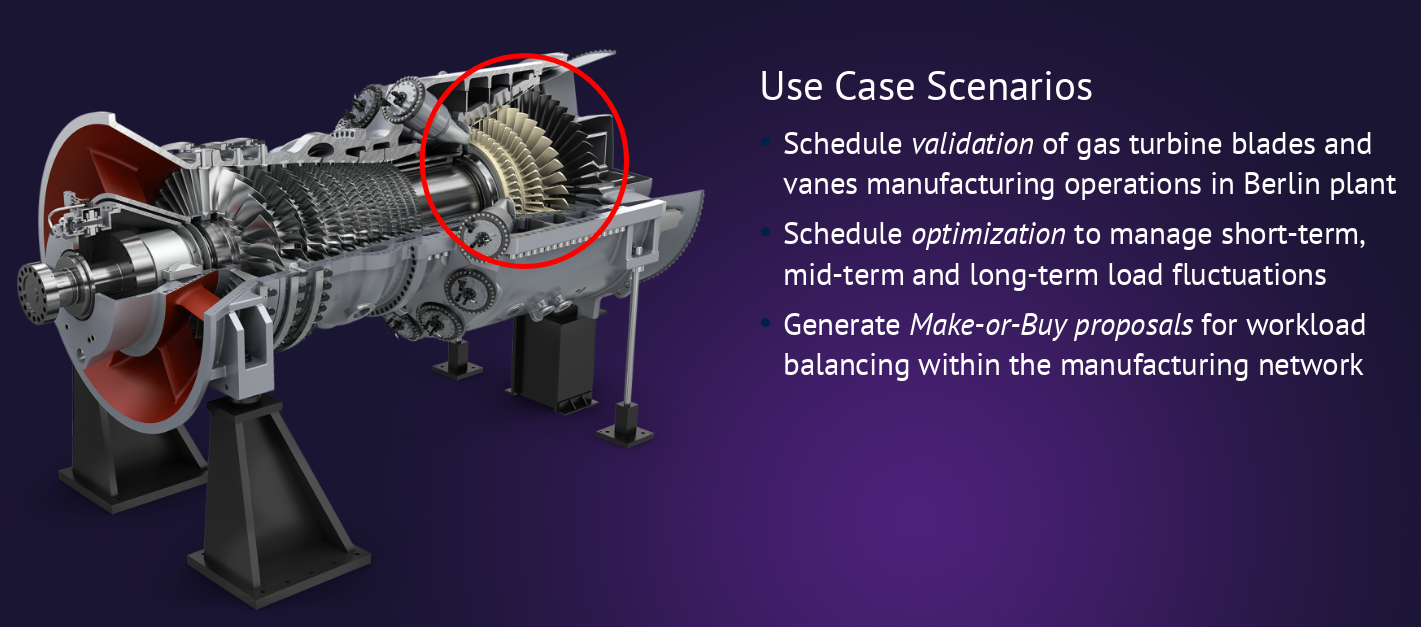
\includegraphics[width=\textwidth]{images/assistantgasturbine}
\end{frame}

\begin{frame}
\frametitle{Digital Twin}
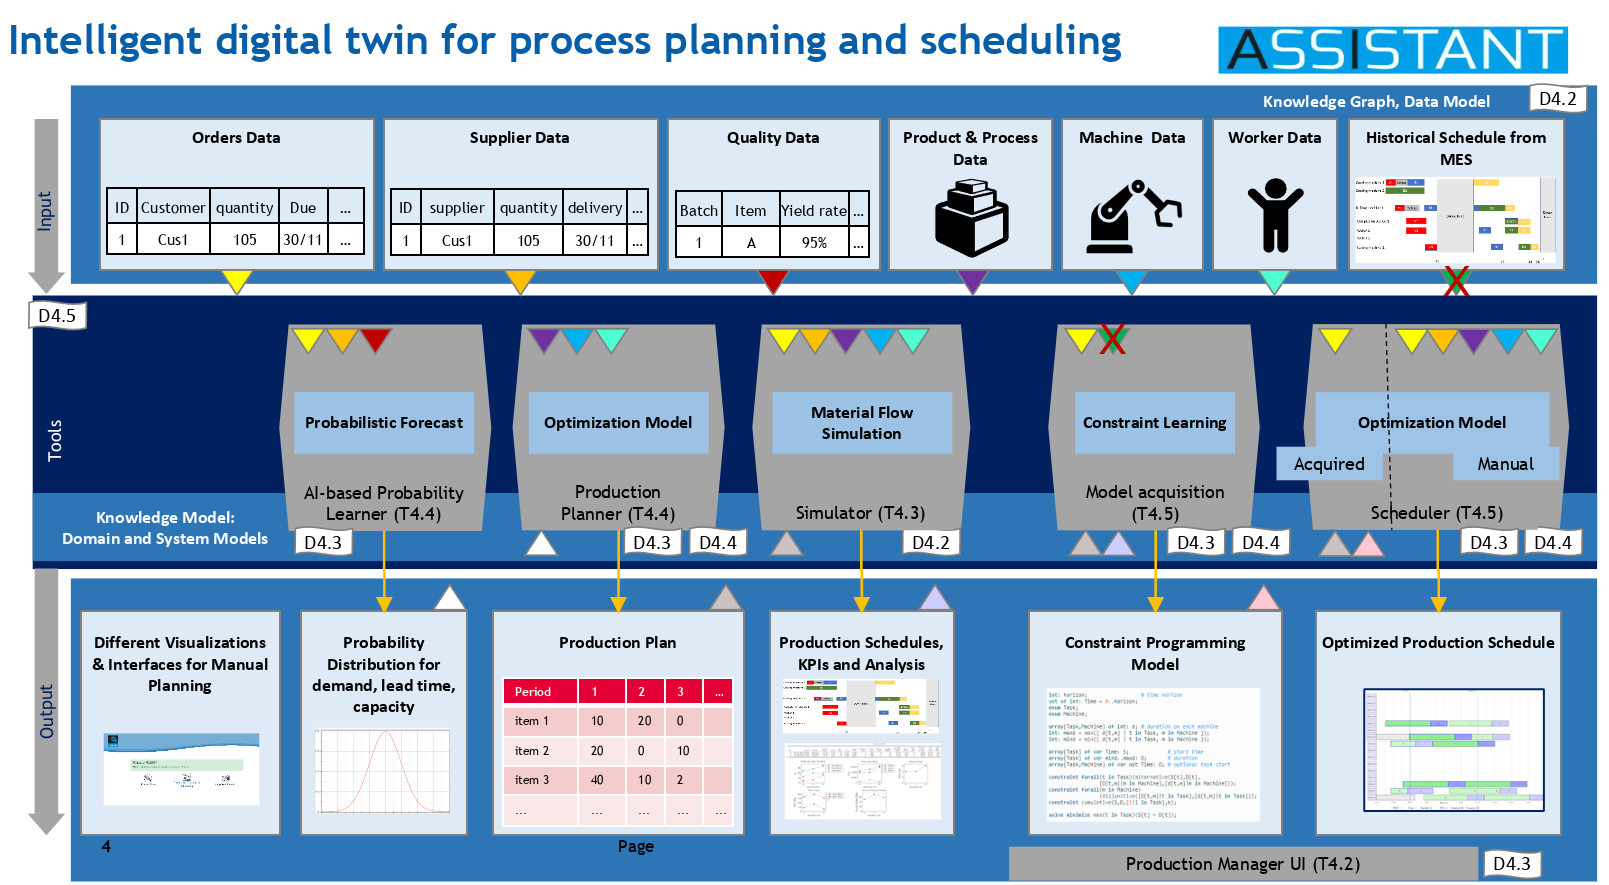
\includegraphics[width=.9\textwidth]{images/assistantdigitaltwin}
\end{frame}

\begin{frame}
\frametitle{SE Product Routing}
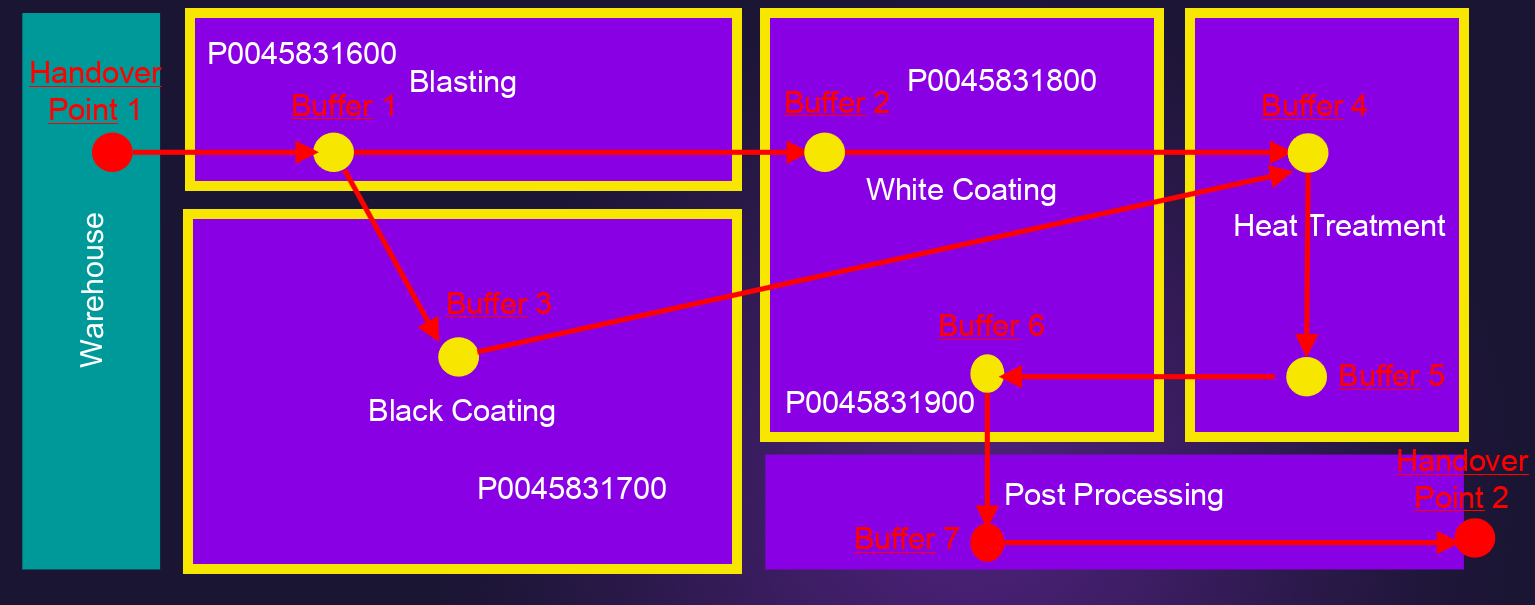
\includegraphics[width=\textwidth]{images/assistantrouting}
\end{frame}

\begin{frame}
\frametitle{Datasets}
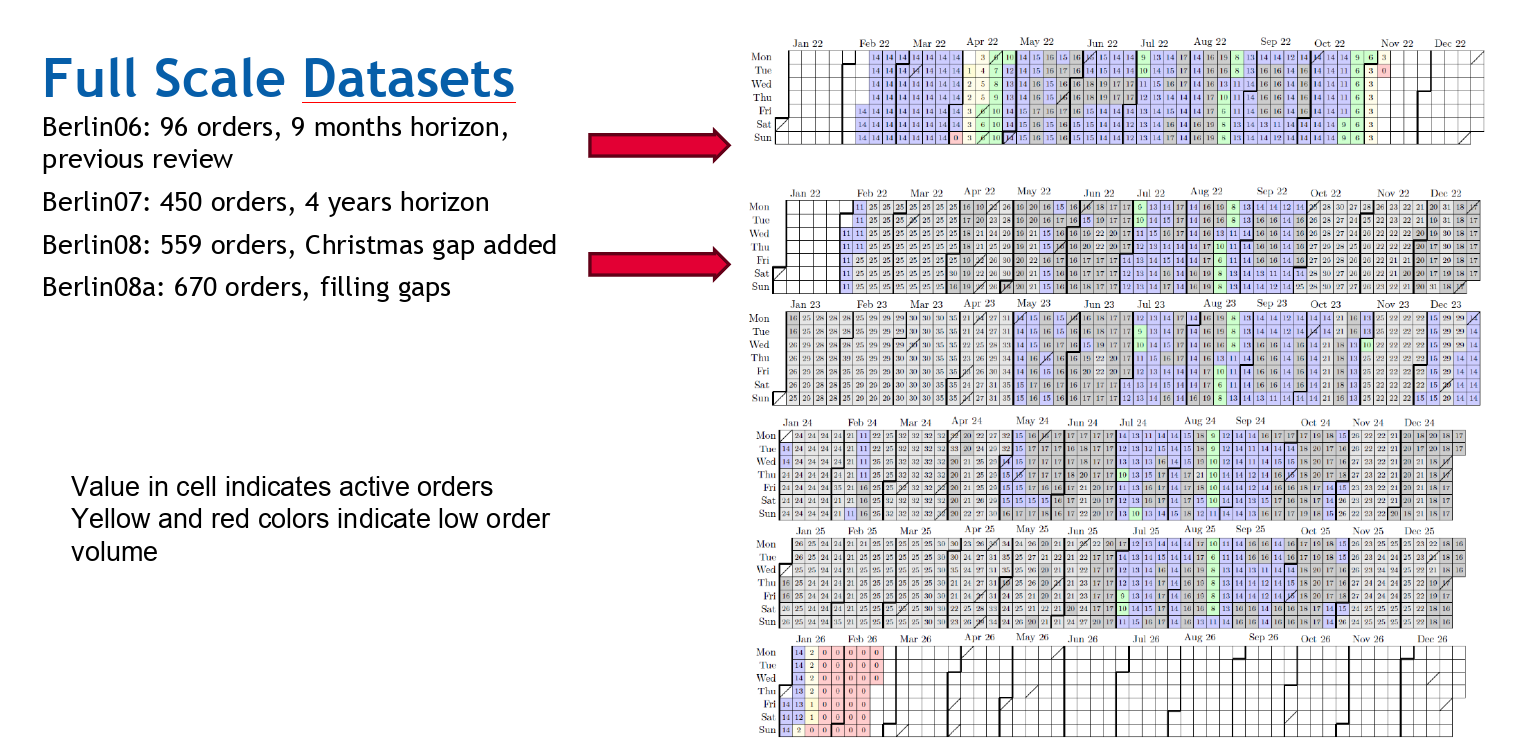
\includegraphics[width=\textwidth]{images/assistantfullscaledatasets}
\end{frame}

\begin{frame}
\frametitle{Optimizer High Level Structure}
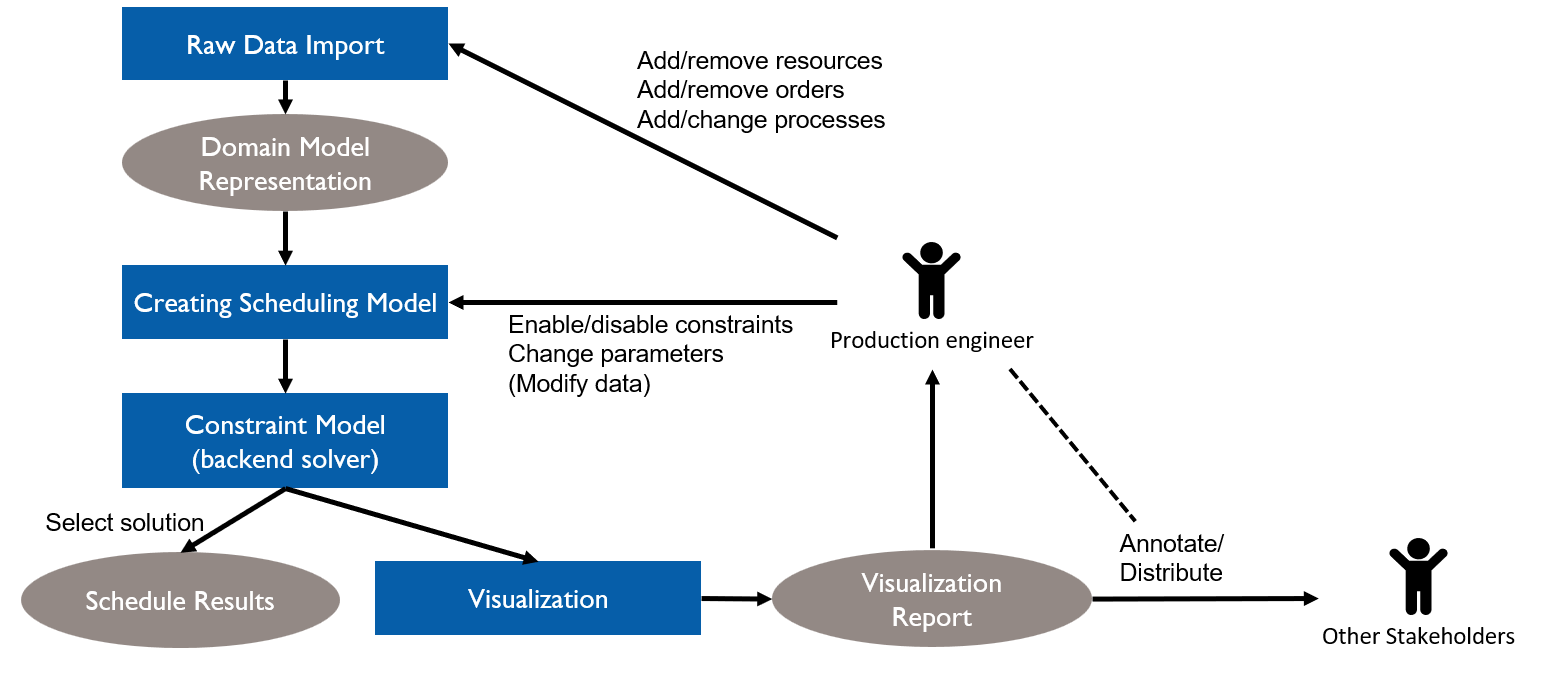
\includegraphics[width=.9\textwidth]{images/overview}
\end{frame}

\begin{frame}
\frametitle{Raw Data - Manual Data Entry Causes Problems}
\begin{columns}
\begin{column}{0.5\textwidth}
\begin{itemize}
\item Raw data come from spreadsheet
\begin{itemize}
\item 20 tabs
\end{itemize}
\item Excel is a particularly bad input data format
\item Realistic, not real data
\item Created by hand/automatically from existing test scenarios
\item Series of files Berlin01 - Berlin05 were too inconsistent to run
\item Berlin06 still contains some errors
\item Optimizer explains all issues that it finds
\end{itemize}
\end{column}
\begin{column}{0.5\textwidth}
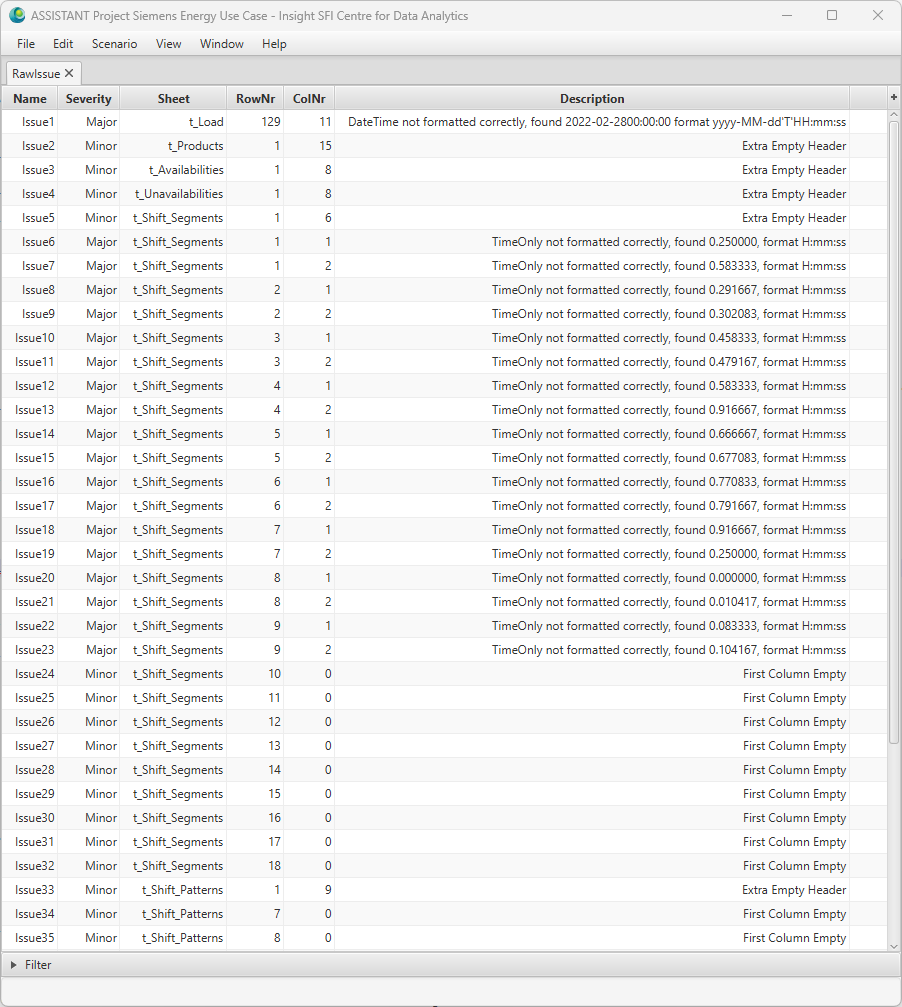
\includegraphics[width=.85\textwidth]{images/rawerror}
\end{column}
\end{columns}
\end{frame}

\begin{frame}
\frametitle{Domain Model - Knowledge Graph}
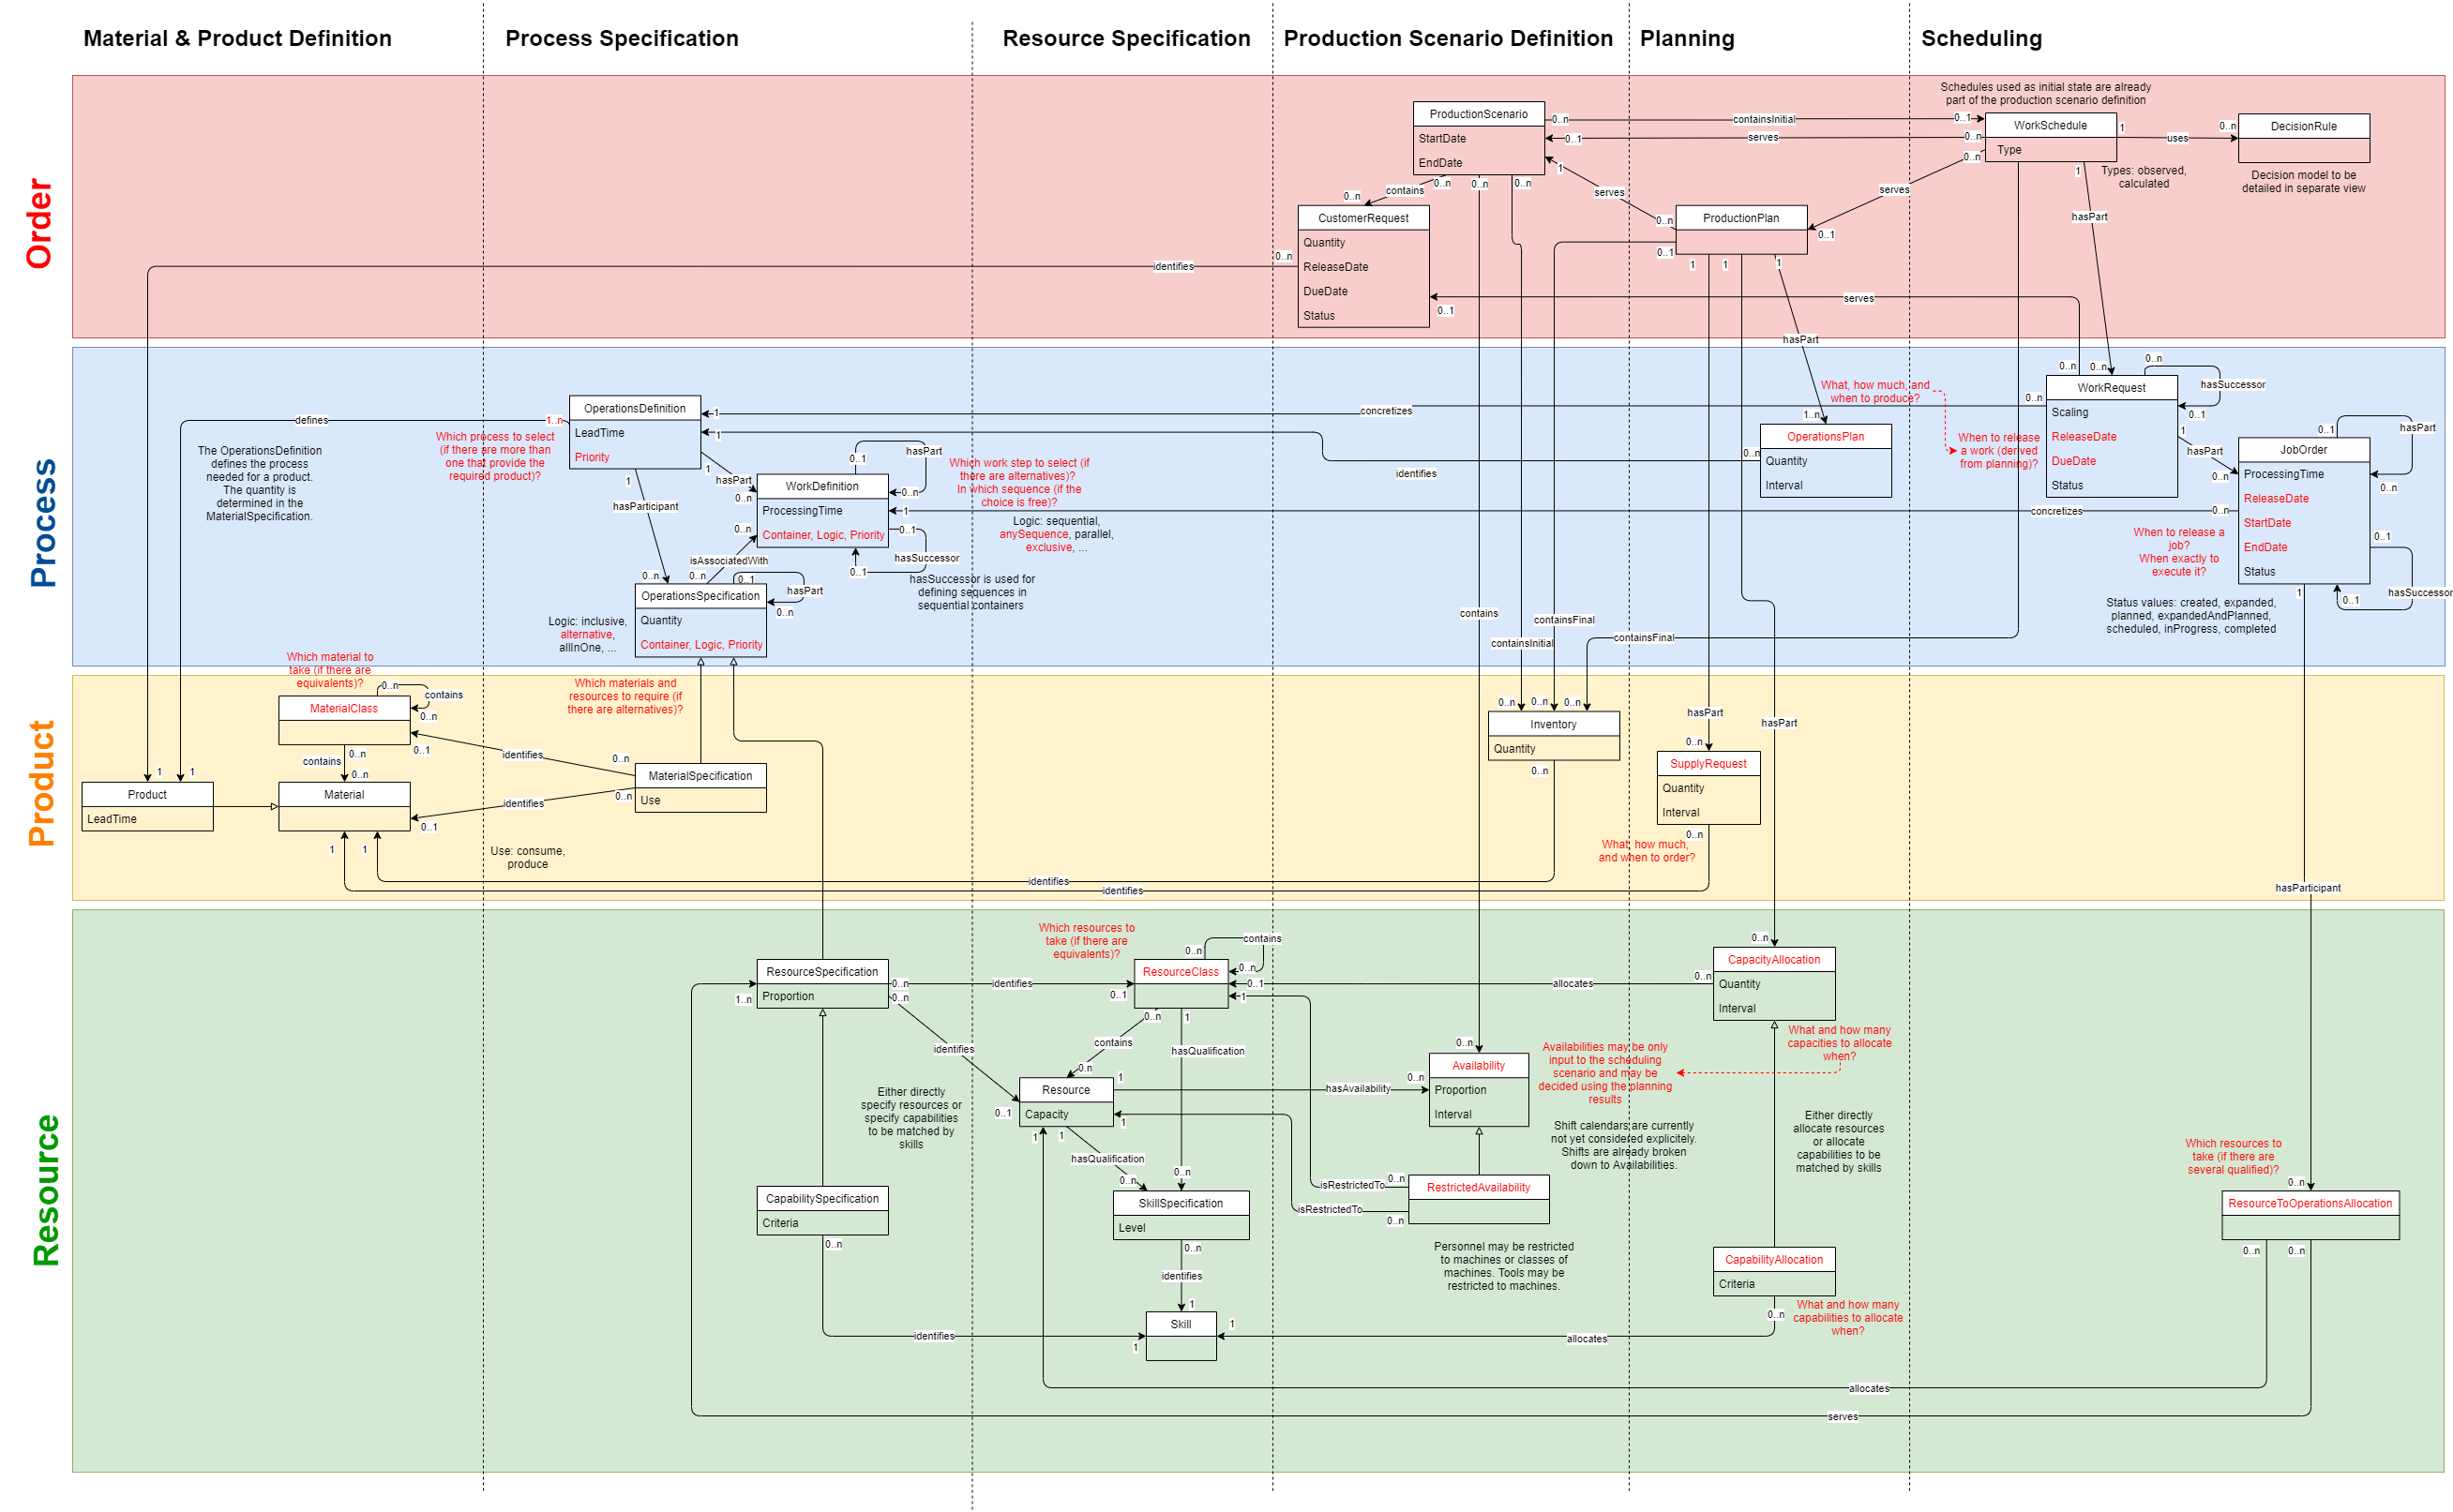
\includegraphics[width=.8\textwidth]{images/DomainModel}
\end{frame}

\begin{frame}
\frametitle{Single Solution for Berlin 08a - Shows Only 20\% of Tasks in Model}
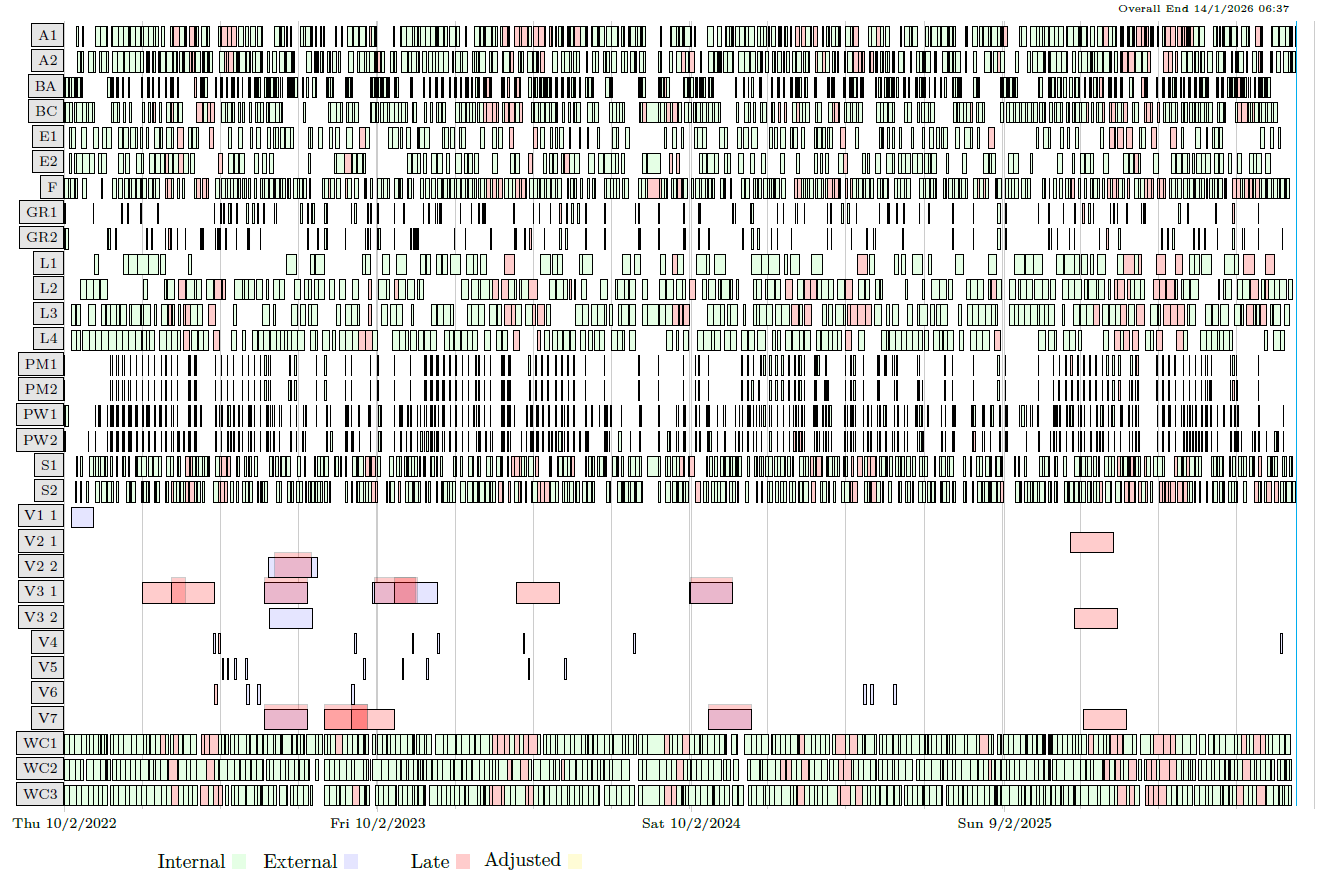
\includegraphics[width=.75\textwidth]{images/solution08apref2}
\end{frame}

\begin{frame}
\frametitle{Challenges for CA}
\begin{itemize}
\item Input data not fully consistent
\item Decide what to do with detected problems
\item Solution only shows active part of schedule
\item Large set of optional tasks not visible as not active
\item Input data contain many fields which are irrelevant for scheduler
\begin{itemize}
\item Component level information
\item Nomenclature
\end{itemize}
\item Many task properties are computed from input data
\begin{itemize}
\item Understand links between multiple objects
\item Time resolution/rounding
\end{itemize}
\end{itemize}
\end{frame}





\section{Conclusion}



\begin{frame}
\frametitle{Summary}
\begin{itemize}
\item Presented different sources for CA benchmarks from simple to complex
\item Few sources present all elements required for CA
\item Benchmarks rather than competition
\item Why data format is important
\item As authors, please provide data, solutions, checkers
\item Algorithms are necessary, but not sufficient for Constraint Acquisition

\end{itemize}
\end{frame}

\begin{frame}
\frametitle{Ad: ACP Winter School 2024}
\begin{itemize}
\item March 25-29, Aussois, France, \url{https://school.a4cp.org/winter2024/} 
\end{itemize}
\includegraphics[width=\textwidth]{images/acpwinterschool}
\end{frame}

\section{Bibliography}

\bibliographystyle{plainurl}
\bibliography{bib,survey}

\end{document}

%%%%%%%%%%%%%%%%%%%%%%%%%%%%%%%%%%%%%%%%%%%%%%%%%%%%%%%%%%%%%%%%%%%%%%%%%%%%%%%%%%%%%%%%%%%%%%%%%



\begin{frame}
\frametitle{}
\begin{tikzpicture}
\end{tikzpicture}
\end{frame}

\begin{frame}
\frametitle{}
\begin{itemize}
\item
\end{itemize}
\end{frame}


\begin{itemize}
\item \textcolor{insight-royalblue}{}
\end{itemize}


\begin{frame}[fragile]
\frametitle{}
\begin{lstlisting}
\end{lstlisting}
\end{frame}

\begin{frame}
\frametitle{}
\begin{columns}
\begin{column}{0.5\textwidth}
\end{column}
\begin{column}{0.5\textwidth}
\end{column}
\end{columns}
\end{frame}

\begin{frame}
\frametitle{}
\begin{columns}
\begin{column}{0.5\textwidth}
\begin{itemize}
\item
\end{itemize}
\end{column}
\begin{column}{0.5\textwidth}
\includegraphics[width=\textwidth]{images/}
\end{column}
\end{columns}
\end{frame}

\begin{frame}
\frametitle{}
\begin{columns}
\begin{column}{0.5\textwidth}
\begin{itemize}
\item
\end{itemize}
\end{column}
\begin{column}{0.5\textwidth}
\begin{itemize}
\item
\end{itemize}
\end{column}
\end{columns}
\end{frame}




\begin{frame}
\frametitle{}
\begin{tikzpicture}
\begin{axis}[ybar,symbolic x coords={},width=\textwidth,height=7cm,ymin=0,xtick=data,ylabel=Count,nodes near coords, nodes near coords align={vertical},enlarge x limits=0.5]
\addplot coordinates{()};
\end{axis}
\end{tikzpicture}
\end{frame}


